
%%%%%%%%%%%%%%%%%%%%%%%%%%%%%%%%%%%%%%%%%%%%%%%%%%%%%%%%%%%%%%%%%%%%%%%
%                           Fourth Chapter                            %
%                       New Posture Generation                        %
%%%%%%%%%%%%%%%%%%%%%%%%%%%%%%%%%%%%%%%%%%%%%%%%%%%%%%%%%%%%%%%%%%%%%%%

\chapter{Posture Generator}
\label{ch:PG}

\graphicspath{{Chapter5-NewPG/Figs/}}

%\section{List of contributions}
%\begin{itemize}
  %\item{Posture Generation, variables and architecture}
    %\begin{itemize}
      %\item Geometric expressions:
        %\begin{itemize}
          %\item Represent everything based on frames
          %\item Automatic derivative computation
        %\end{itemize}
      %\item Automatic mapping
      %\item Problem generator: a posture generation problem factory
    %\end{itemize}
  %\item{Problem Formulation: formulation of usual problems in the geometric expressions framework}
    %\begin{itemize}
      %\item Contact with plane surface
      %\item Static equilibrium: Newton/CoM projection
      %\item Forces in friction cones
      %\item Articular limits
      %\item Torque limits
      %\item Torque minimization
      %\item Goal Posture
    %\end{itemize}
  %\item{Implementation of new types of constraints in our formulation}
    %\begin{itemize}
      %\item Contact with parametrized surfaces on Rn
      %\item Contact with parametrized surfaces on S^2: Sphere, SuperEllipsoid
      %\item Contact with Catmull-Clark Subdivision surfaces
    %\end{itemize}
  %\item{Contact with desired force}
  %\item{Potential contacts}
  %\item{Simulation Results}
  %\item{Multi-Robot}
%\end{itemize}

Writing a posture generation problem can easily become cumbersome without the appropriate tools.
Common pitfalls are for example writing the derivative of a function, managing how the Jacobian matrices of the already implemented functions are modified when a variable is added to the problem, adding a new type of constraint, or correctly writing a function on a sub-manifold of the problem manifold.
A fair amount of bookkeeping is always necessary, which should not be the charge of the user writing the constraints.
In our PG, we propose an architecture automating most of the burdensome tasks so that the user can focus on the mathematical formulation of the problem:
\begin{itemize}
  \item A system of geometrical and mathematical expression trees that automatically computes the mathematical expressions behind the geometric relations;
  \item An automatic mapping between the submanifold of each function and the global manifold of the problem;
  \item A problem generator that aggregates all the information from the above-mentioned items to generate an optimization problem that can be passed to the solver.
\end{itemize}
We then propose an extension to classic posture generation by developing a constraint of contact with parametrized surfaces which takes advantage of our framework.


%%%%%%%%%%%%%%%%%%%%%%%%%%%%%%%%%%%%%%%%%%%%%%%%%%%%%%%%%%%%%%%%%%%%%%%
%                        GEOMETRIC EXPRESSIONS                        %
%%%%%%%%%%%%%%%%%%%%%%%%%%%%%%%%%%%%%%%%%%%%%%%%%%%%%%%%%%%%%%%%%%%%%%%

\section{Geometric expressions}
\label{sec:geometric_expressions}

Most of the robotic posture generation constraints are geometric.
In order to simplify the writing of functions, we use a dedicated system of expression graph encapsulated in a set of geometric objects.
The main idea is to separate the purely mathematical logic from the geometric one.
As an example, if $P_r$ and $\overrightarrow{V_r}$ are a point and a vector attached to the camera of the robot, and $P_e$ is a fixed point in the environment, the constraint $(P_e - P_r)\cdot \overrightarrow{V_r} = 0$ can be used to have the robot's camera directed toward $P_e$.
With our implementation, the user creates only those objects and write the code \texttt{(Pe-Pr).dot(Vr)} to create the needed task function.
The geometric layer ensures that all the quantities are expressed in the correct frame, the mathematical layer performs the corresponding operations.
If $q$ is a variable object, \texttt{(Pe-Pr).dot(Vr).diff(q)} returns automatically the differential of the expression w.r.t. $q$. This makes the writing of the constraints very easy.

At the mathematical level, we consider 5 types of expressions which can be either variables or constants:
\begin{itemize}
  \item Scalar, a 1-dimensional element of $\mathbb{R}$
  \item Coordinates, a 3-dimensional element of $\mathbb{R}^3$
  \item Rotation, a $3\times3$ matrix representing a 3D rotation
  \item Transformation, a $4\times4$ matrix representation of a 3D isometry
  \item Array, a dynamic size array
\end{itemize}
The meaningful unary (inverse, opposite, norm...) and binary (multiplication, addition, subtraction, dot product...) operations (with their derivatives by chain rule) are implemented.
We also have a Function class for more complex expressions, for example expressing $q \mapsto T_i(q)$ where $T_i$ is the transformation between the reference frame of the robot and the frame of its $i$-th body\footnote{The kinematics of rigid body systems is handled by the RBDyn library (\url{git@github.com:jrl-umi3218/RBDyn.git})}.
The combinations of those elementary operations define a computation graph, just like in many symbolic calculation frameworks.

Each expression is able to compute its own value and the value of its derivative with respect to another expression.
For example, let $A$ and $B$ be two unrelated expressions.
We denote $\dim(x)$ the dimension of expression $x$.
The value of expressions $A$ or $B$ are obtained by respectively calling the methods {\tt A.value()} and {\tt B.value()}.
The derivative of $A$ with respect to itself is obtained by calling the method {\tt A.diff(A)} and returns an Identity matrix of size $\dim(A)$.
Whereas the derivative of $A$ w.r.t $B$ returns a zero matrix with $\dim(A)$ rows and $\dim(B)$ columns.
\begin{equation}\nonumber
  \frac{\partial A}{\partial A} = \mathbf{1}_{\dim(A)}, \quad \frac{\partial A}{\partial B} = \mathbf{0}_{\dim(A),\dim(B)}
\end{equation}

Each operator on expressions defines its resulting expression, thus, it defines a {\tt value} and a {\tt diff} methods.
For example, let us consider that $A$ and $B$ are 3D coordinate expressions and a new expression $C = A\cdot B$ that is defined as the dot product of $A$ and $B$, in code, one can write C's definition as simply:
\begin{center}
{\tt Scalar C = dot(A,B)}.
\end{center}
The value and the derivative of $C$ w.r.t any $x$ expression are then automatically computed as follows:
\begin{equation}
\label{eq:dot}
  C = A\cdot B,\quad \frac{\partial C}{\partial x} = A^T\frac{\partial B}{\partial x} + B^T\frac{\partial A}{\partial x}
\end{equation}

%\begin{table}
%\begin{tabular}{cc}
  %\toprule
  %$C = A\cdot B$ & {\tt C.value() = dot(A.value() + B.value())} \\
  %\midrule
  %$\frac{\partial C}{\partial x} = A^T\frac{\partial B}{\partial x} + B^T\frac{\partial A}{\partial x}$ & {\tt C.diff(x) = A.value().transpose()*B.diff(x) \\ + B.value().transpose()*A.diff(x)} \\
  %\bottomrule
%\end{tabular}
%\end{table}

The code of the dot function that translates eq:~\Eqref{eq:dot} is pretty straightforward:
\begin{center}
{\tt C.value() = A.value().dot(B.value())\\
C.diff(x) = A.value().transpose()*B.diff(x) \\ + B.value().transpose()*A.diff(x)}
\end{center}

It is easy to extend the capabilities of this framework by implementing additional operations.
By following this approach, we can easily compute the values and derivatives of expressions that are the outcome of complex arithmetic trees.
Currently, the following binary operators are available: cross product, dot product, classic product, addition, subtraction, transformation.
And the following unary operators are available: component extraction, inverse, norm, rotation, square root, transformation, and vectorization.

The geometric layer consists of physical or geometric objects, called features, which exist independently of their mathematical expression in a given reference frame.
We have so far four objects:
\begin{enumerate}
  \item A Frame, defined by a Transformation expression and a reference frame.
  \item A Point, defined by a Coordinates expression and a reference frame.
  \item A Vector, defined by a Coordinates expression and a reference frame.
  \item A Wrench, defined by a pair of Coordinates expressions and a reference frame.
\end{enumerate}
We have a special World Frame object to serve as starting reference frame.

For each feature, one can get its expression in a given frame.
Basic operations are defined between those features (when applicable).
For example, the subtraction between two Points gives a Vector.
The geometric logic resides in the change of frame and those operations.

Based on that expression system, the robot's geometry can simply be represented by a set of frames representing all its links, and functions that keep track and update the transformations of the frames of all its bodies, with respect to an Array expression on entry, its articular parameters.
The forward kinematics Algorithm~\ref{alg:FK} and the Jacobian computation Algorithm~\ref{alg:jacobian_computation} are used to define those functions.
For a given articular parameter array, the user can query the frame of any body on the robot, and by composition, any feature defined on a frame of the robot, as well as its derivatives.
This tool allows for a simplified writing of robotics constraints as a combination of operations on geometric features, without worrying about the vectors and matrices and without having to write the derivatives.

Let us consider a simple constraint and its expression in this framework:
we define a point $P_h$ on a body of a robot and a point $P_e$ in the environment.
We want to write a constraint that ensures that $P_h$ and $P_e$ match.
%We can write that constraint by requiring that the vector defined by $V = P_h - P_e$ is zero, which means that the 3 elements of the expression of $V$ in a given frame $F$ are zero.
Given a frame $F$, we can simply write that as:
\begin{center}
\tt{ P\_h.coord(F) - P\_e.coord(F)=0}
\end{center}
(the "$=0$" part of the equation is here for readability only; in the code, the value of the resulting expression is constrained by boundaries)

In the case of a scalar expression like $(P_e - P_r)\cdot \overrightarrow{V_r} = 0$, it can be written without any consideration about frames as
\begin{center}
{\tt(P\_h - P\_e).dot(V) = 0}.
\end{center}

This mathematical and geometric expression framework simplifies the task of the constraints developers.
And it helps to avoid calculation mistakes because one only needs to write the code for elementary functions and their combination is computed automatically by chain rule.


%%%%%%%%%%%%%%%%%%%%%%%%%%%%%%%%%%%%%%%%%%%%%%%%%%%%%%%%%%%%%%%%%%%%%%%
%                          AUTOMATIC MAPPING                          %
%%%%%%%%%%%%%%%%%%%%%%%%%%%%%%%%%%%%%%%%%%%%%%%%%%%%%%%%%%%%%%%%%%%%%%%

\section{Automatic mapping}
\label{sec:automatic_mapping}

The manifold $\mathcal{M}$, on which the optimization takes place, is a Cartesian product of several sub-manifolds. Same goes for their representation spaces:
\begin{align}
  \begin{split}
    \mathcal{M}& = \mathcal{M}_1\times\mathcal{M}_2\times\mathcal{M}_3\times\hdots\\
    \mathbb{E}& = \mathbb{E}_1\times\mathbb{E}_2\times\mathbb{E}_3\times\hdots
  \end{split}
\end{align}
From the solver's viewpoint, the entry space of each function is the complete manifold.
But for the developer, writing a function on the complete $\mathbb{E}$ is cumbersome because (i) of the need to manage indexes, and (ii) when the function is implemented, the complete $\mathbb{E}$ may not be known.
A user-written function $f$ is usually defined on a subset of $\mathbb{E}$, say $\mathbb{E}_I=\mathbb{E}_i\times\mathbb{E}_j\times\mathbb{E}_k\hdots$, that is minimalistic for that function, and should not account for unrelated manifolds.
One does not want to think about the values of the forces when writing a geometric constraint for example.

We developed an automatic mapping tool that keeps track of all the necessary mappings for each function added and upon the instantiation of the problem, generates the correct projection functions $\pi_I$ such that the developer can write a function $f$ on $\mathbb{E}_I$ while the solver receives it as a function $f \circ \pi_I$ on $\mathbb{E}$.

This tool was built as an add-on to the RobOptim~\cite{moulard:jsme:2013} framework called {\bf roboptim-core-manifold} and its goal is to extend the notion of function to take into account its application manifold and map the correspondence between the values in the input of the problem and the input of the function.
We define a class called DescriptiveWrapper that contains a RobOptim function and a description of its application manifold.
Once a function is wrapped in a DescriptiveWrapper and the optimization problem is set, we need to establish the mapping between the variable of the problem, which is defined on the global manifold of the problem, and the input of the function that must match the description of its application manifold.
That is the role fulfilled by the WrapperOnManifold layer, that compares the two manifolds, matches them and computes an input mapping from the problem's input vector to the function's, which we denote $\pi_I$.
This mapping is computed once during the instantiation of the problem and then used at each call of the function.
The use of the input mapping is illustrated by the example in~\Figref{fig:auto_map}
%\begin{equation}
  %\begin{split}
  %\pi_I:\mathbb{E}\to\mathbb{E}_I\\
  %f:\mathbb{E}_I\to\mathbb{R}\\
  %f\circ\pi_I:\mathbb{E}\to\mathbb{R}
  %\end{split}
%\end{equation}

\begin{figure}[!htb]
\centering
  \centering
  \setlength\fboxsep{0pt}
  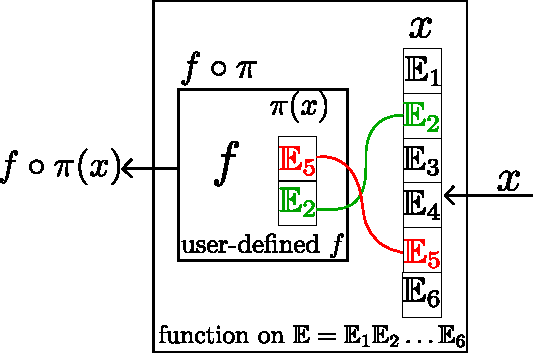
\includegraphics[width=.5\linewidth]{auto_mapping_text.pdf}
\caption{automatic variable mapping}
\label{fig:auto_map}
\end{figure}

%%%%%%%%%%%%%%%%%%%%%%%%%%%%%%%%%%%%%%%%%%%%%%%%%%%%%%%%%%%%%%%%%%%%%%%
%                        PROBLEM FORMULATION                          %
%%%%%%%%%%%%%%%%%%%%%%%%%%%%%%%%%%%%%%%%%%%%%%%%%%%%%%%%%%%%%%%%%%%%%%%

\section{Problem formulations}
\label{sec:problem_formulations}

Let $q=[q_F^T; q_r^T]\in SE(3)\times \mathcal{M}_r$ be the combination of the free-flyer of the robot $q_F\in SE(3) = \mathbb{R}^3 \times SO(3)$ and the articular parameters $q_r\in\mathcal{M}_r$.
Let $\mathcal{W}_i(p)=\{f_i,m_i(p)\}$ be the wrench (force+moment) applied by the environment onto the robot at contact $i$ and expressed on point $p$.
A frame $F$ is composed of a reference point and an orthonormal basis of 3 vectors $F = \{O, (\vec{x}, \vec{y}, \vec{z})\}$.
For frames define on a surface, with one vector of $(\vec{x}, \vec{y}, \vec{z})$ being the outbound normal to the surface, and the two others tangent, we rename $\vec{n}$ the normal one and $\vec{t}, \vec{b}$ (tangent and bitangent) the two other ones, ensuring that $(\vec{n}, \vec{t}, \vec{b})$ is an orthonormal direct basis.
When a frame is denoted with the subscript i, $F_i$, all its components are added the same subscript.

Here is a list of constraints that we consider in our problems:

\begin{itemize}
\item Joint limits ${q^-} \leq q_r \leq {q^+}$:\\
These cannot be directly translated on manifolds other than $\mathbb{R}^n$.
For example, spherical joints can be parametrized on $S^2 \times \mathbb{R}$, then the $S^2$ part can be limited by a cone, and the $\mathbb{R}$ part can have real bounds (in that case the limit constraint is not a simple bound constraint, but writes as $f(q_r)\leq 0$).

%\item The contact constraint consists in identifying the features of two frames $F_1$ and $F_2$.
%For example, for a planar contact, we can write the constraints~\Eqref{eq:planar_contact_bad}.
%\begin{equation}
  %\left\{
  %\begin{array}{ll}
    %\overrightarrow{O_1O_2}\cdot\vec{n_1} = 0\\
    %\vec{n_2} = -\vec{n_1} \\
  %\end{array}
  %\right.
%\label{eq:planar_contact_bad}
%\end{equation}
%In practice, for a better numerical behavior of the optimization, we write that $\vec{n_2}$ is perpendicular to the plan $\{O_1, \vec{t_1}, \vec{b_1}\}$ and has opposite direction with $\vec{n_1}$,~\Eqref{eq:planar_contact}:
%\begin{equation}
  %\left\{
  %\begin{array}{ll}
    %\overrightarrow{O_1O_2}\cdot\vec{n_1} = 0\\
    %\vec{n_2}\cdot\vec{n_1} \leq 0 \\
    %\vec{n_2}\cdot\vec{t_1} = 0 \\
    %\vec{n_2}\cdot\vec{b_1} = 0
  %\end{array}
  %\right.
%\label{eq:planar_contact}
%\end{equation}
%Note that on $F_2$ only the point $O_2$ and the vector $\vec{n_2}$ are necessary.
%Other types of contacts can be created that way, by equalizing other features, as explained in~\cite{escande:ras:2013}.
%For example, we can fix the contact to a given position and orientation by adding to it the following set of equation~\Eqref{eq:fix_planar_contact} that locks the degrees of freedom of rotation around the normal and translation in the tangent plane of the contact:
%\begin{align}
  %\left\{
  %\begin{array}{ll}
    %\overrightarrow{O_1O_2} \cdot \vec{t_1} = 0 \\
    %\overrightarrow{O_1O_2} \cdot \vec{b_1} = 0 \\
    %\vec{b_2} \cdot \vec{t_1} = 0 \\
    %\vec{t_2} \cdot \vec{b_1} = 0 \\
    %\vec{t_2} \cdot \vec{t_1} \leq 0
  %\end{array}
  %\right.
%\label{eq:fix_planar_contact}
%\end{align}
%Those two sets of equations~\Eqref{eq:planar_contact} and~\Eqref{eq:fix_planar_contact} can easily be recombined to generate other types of constraints (e.g.\ fixing only the translation, or only the rotations\ldots).

\item The Frame constraint is a generic type of constraint which consists in blocking a predefined set of degrees of freedom of one frame $F_2$ w.r.t. another frame $F_1$.
By default, the frame $F_2$ has 6 degrees of freedom w.r.t. $F_1$, three translational degrees of freedom TX, TY, and TZ, respectively along $\vec{x_1}$, $\vec{y_1}$ and $\vec{z_1}$ and three rotational ones RX, RY, and RZ, respectively around $(O_1,\vec{x_1})$, $(O_1,\vec{y_1})$ and $(O_1,\vec{z_1})$.
We can write constraints such that any combination of the translational degrees of freedom is blocked:

\begin{align}
  \text{If TX is blocked: } \overrightarrow{O_1 O_2} \cdot \vec{x_1} = 0 \\
  \text{If TY is blocked: } \overrightarrow{O_1 O_2} \cdot \vec{y_1} = 0 \\
  \text{If TZ is blocked: } \overrightarrow{O_1 O_2} \cdot \vec{z_1} = 0
\end{align}

Similarly, any pair of rotational degrees or the three of them can be blocked (blocking only one rotation is not possible with that formalism).
If the three rotations RX, RY, RZ are blocked, we get the set of constraints~\ref{eq:3_rotations_blocked}:
\begin{equation}
\label{eq:3_rotations_blocked}
\begin{cases}
  \vec{z1}\cdot\vec{y2} = 0 \\
  \vec{z1}\cdot\vec{x2} = 0 \\
  \vec{x1}\cdot\vec{y2} = 0 \\
  \vec{z1}\cdot\vec{z2} \geq 0 \\
  \vec{y1}\cdot\vec{y2} \geq 0
\end{cases}
\end{equation}

When two rotational degrees of freedom are blocked, we get the set of constraints~\ref{eq:2_rotations_blocked}
To generalize the following formulas, we rename the axis X, Y, and Z with respect to their respective roles in this constraint.
The one rotational degree that remains free is denoted N with vector $\vec{n}$, and the two others are denoted T and B, with vectors $\vec{t}$, and $\vec{b}$.
Those 3 vectors are ordered such that $(\vec{n}, \vec{t}, \vec{b})$ is an orthonormal direct basis.

\begin{equation}
\label{eq:2_rotations_blocked}
\begin{cases}
  \vec{n_2}\cdot\vec{n_1} \geq 0 \\
  \vec{n_2}\cdot\vec{t_1} = 0 \\
  \vec{n_2}\cdot\vec{b_1} = 0
\end{cases}
\end{equation}

In theory, one could simply write that constraint as $\vec{n_1}=\vec{n_2}$, but in practice, this formulation leads to bad numerical behavior of the optimization, thus we prefer~\ref{eq:2_rotations_blocked}.

All those independent sets of constraints can be combined to create a wide variety of geometric constraints.
For example, one can create a mobile planar contact constraint with normal $\vec{z}_1$ by blocking TZ, RX and RY.
A punctual contact constraint can be devised by blocking TX, TY and TZ.
To completely fix the position of $F_2$ w.r.t. $F_1$, one can block TX, TY, TZ, RX, RY, and RZ.
And many other types of custom constraints can be devised with this formulation.

In the event that the two frames do not have a satisfying configuration to write the desired constraint with this formalism (for example, if one wants to write a planar contact between two surfaces $S_1$ and $S_2$, where $\vec{z_1}$ and $\vec{z_2}$ are outbound normal vectors, then equation~\ref{eq:2_rotations_blocked} is not satisfactory because we want to oppose $\vec{z_1}$ and $\vec{z_2}$, not identify them).
Then the user defines a new frame $F_2'$ that is a constant 3D transformation away from $F_2$ (in that case a rotation of $\pi$ around $(O_1,\vec{x_1})$ would suffice).

\item The stability constraint ensures that the Euler-Newton equation~\Eqref{eq:NewtonWrench} is balanced for the set of external wrenches applied to the robot (gravity $\mathcal{W}_G$ and contact forces $\mathcal{W}_i$).
\begin{equation}
  \sum_{i}{\mathcal{W}_i(p)} + {\mathcal{W}_G(p)} = 0
  \label{eq:NewtonWrench}
\end{equation}
For each contact that bears forces (`stability' contact), a wrench applied on the robot at the contact point is added to the problem.
If the contact is added through a frame constraint between $F_1$ and $F_2$, the wrench can be formed by a combination of elementary components that are:
\begin{itemize}
\item FX: force along $\vec{x_1}$, value $f_x$
\item FY: force along $\vec{y_1}$, value $f_y$
\item FZ: force along $\vec{z_1}$, value $f_z$
\item MX: moment around $(O_1,\vec{x_1})$, value $m_x$
\item MY: moment around $(O_1,\vec{y_1})$, value $m_y$
\item MZ: moment around $(O_1,\vec{z_1})$, value $m_z$
\end{itemize}
That wrench is parametrized on a $\mathbb{R}^m$ with $m$ the number of components used.
%For punctual contacts, the moment part is null on the application point.
%Only a parametrization of the force part on $\mathbb{R}^3$ is needed.
We model the resultant wrench of planar contacts as a combination of punctual forces applied at each vertex of the contact polygon.
In the case of interaction forces between 2 robots, only one wrench is created and it is used as is in the stability equation of one robot and its opposite is used for the stability of the second robot.
That way, we are guaranteed that the forces in between the robots are balanced and we can evaluate the stability of each robot separately.

\item The friction cone constraint can be used to limit the tangential part of any force to avoid slippage.
We write it as~\Eqref{eq:friction} (with $\mu$ the friction coefficient)
\begin{equation}
  \begin{split}
    \mu^2f_z^2-f_x^2-f_y^2 \geq 0 \\
    f_z \geq 0
  \end{split}
  \label{eq:friction}
\end{equation}

\item The rotational friction limit constraint can be used to limit the friction torque of any force to avoid slippage.
We write it as~\Eqref{eq:frictionTorque} (with $\sigma$ the rotational friction coefficient)
\begin{equation}
  \begin{split}
    \sigma^2f_z^2-m_z^2 \geq 0 \\
    f_z \geq 0
  \end{split}
  \label{eq:frictionTorque}
\end{equation}


\item The collision avoidance constraint can be defined between any two bodies.
A convex mesh is attached to each body involved in the constraint.
We denote them $C_1$ and $C_2$.
We use the {\tt sch-core} library described in~\cite{benallegue:icra:2009} that implements an efficient GJK algorithm to compute the distance $d(C_1,C_2)$ between 2 convex shapes and its derivative.
A description of strictly convex hulls that can be used for this purpose is detailed in~\cite{escande:itro:2014}.
For each collision avoidance constraint, we require that the distance between the two convex remains superior to a minimal distance $d_{\min}$
\begin{equation}
  d(C_1, C_2)\geq d_{\min}
\end{equation}

\item The torque limit constraint makes use of the Inverse Statics Algorithm~\ref{alg:ISmatrix} to compute the torques in all the joints of every robots and their derivatives are computed by Algorithm~\ref{alg:TJC}.
Denoting $\tau_i$ the torque in joint $i$ resulting from the robot's configuration and the external forces applied on it, and its lower and upper limits as $\tau_i^-$ and $\tau_i^+$.
The torque limit constraint writes as follows:
\begin{equation}
  \forall i,\ \tau_i^- \leq \tau_i \leq \tau_i^+
\end{equation}
\end{itemize}


%The frame in which the constraints are written matters critically.
Most often, the frame's configuration depends on a part of the optimization variables, that must be accounted for in computing the constraints' Jacobian.
Our framework computes such dependencies automatically.

Another important part is the problem's cost function.
Any function of the problem's variables that returns a scalar value can be used as a cost function.
In our formulation, we take a sum of cost functions into account, several different functions $f_i$ over different variables can be defined separately.
And then combined in a weighted sum as the problem's cost function (with $w_i$ the weight of function $f_i$):
\begin{equation}
  cost = \sum\limits_i w_i f_i
\end{equation}
Taking advantage of our framework, the set of variables over which the cost function is defined, its value and its derivatives are then computed automatically.

A typical cost function is the distance to a reference posture $q_0$.
On a robot that has all its articulations parametrized on $\mathbb{R}$ the distance can be expressed simply with the Euclidean norm $d = \norm{q_r-q_0}^2$.
Since we work on non-Euclidean manifolds, the logarithm function on the manifold must be used.
It gives the distance vector between two points in the tangent space, the norm of this vector can be used as a distance.
So we get $d = \norm{\text{log}_{q_0}(q_r)}^2$ (note that on $\mathbb{R}^n$, $\norm{\text{log}_{q_0}(q_r)}^2 = \norm{q_r - q_0}^2$)

We can also use the cost function to set a target value $v$ for the value of a contact force $\vec{F}$ in a given direction $d$. By simply implementing the following function:
\begin{equation}
  f = \norm{\vec{F}\cdot\vec{d}-v}
\end{equation}

The list of constraints and cost functions that can be used in robotics posture generation problems can be extended, and this process is made easier by our framework.


%%%%%%%%%%%%%%%%%%%%%%%%%%%%%%%%%%%%%%%%%%%%%%%%%%%%%%%%%%%%%%%%%%%%%%%
%                           IMPLEMENTATION                            %
%%%%%%%%%%%%%%%%%%%%%%%%%%%%%%%%%%%%%%%%%%%%%%%%%%%%%%%%%%%%%%%%%%%%%%%

\section{Implementation}
\label{sec:implementation}

In this section, we provide an overview of some of the key elements of the framework:

\paragraph{Problem's configuration:}
The implementation of the core structure of a posture generation problem is written in \texttt{C++}.
A text file in YAML format can be used to configures the solver and some custom parameters of the problem; It is parsed at runtime to avoid having to recompile the problem for every configuration change.
Also, some \texttt{Python} bindings have been developed to allow writing the core structure of the problem without compilation.
%We use two types of configuration files:
%\begin{itemize}
  %\item A default configuration file contains all the usual data, like the paths to robots description directories, as well as some data about each robot, like the lists of usual self-collisions used per robot, etc\ldots\\ {\tt problem-generator/configs/problemGeneratorConfig.yml.in}
  %\item A problem specific configuration file that contains all the data necessary to describe the problem, like the list of robots, the location of some geometric features, some solver parameters, the choice for a robot to have a fixed basis, or torque limits and anything else that can help specify the problem.
%\end{itemize}

\paragraph{The Robot class:}
%It is instantiated from a Robot::Init structure that contains all the necessary data for its construction.
%Which includes its name, its URDF path, the path of its collision meshes, some booleans defining if the robot is fixed, has torque limits, etc\ldots
%On instantiation of a robot, we use this URDF to instantiate the RBDyn objects that are used to compute the Forward Kinematics and Inverse Statics of the robot: a MultiBody, a MultiBodyGraph and a MultiBodyConfig, as well as its joint, torque limits, and the manifold in which the variables of the robot live.
%The robot object is equipped with an external\_forces object that handles the external forces applied to it, and a torques object that handles its joint torques.
%A Frame is created on each of the bodies of the robot.
%A set of predefined surfaces on bodies can be loaded from an rsdf file.
%A set of collision convex meshes attached to the bodies of the robot is created based on a provided list of mesh files.
%The configuration of a robot depends on its articular parameters, to hanble that, the robot object contains an update method that runs the Forward Kinematics algorithm and updates the transformations of each body and its jacobian, which, by extension updates the its body frames. Every body frames get their transformation's values and derivatives from those quantities.
The RBDyn library contains all the low-level tools and algorithm to compute the kinematics and statics of a robot.
The robot class is built on top of RBDyn to provide high-level functionalities while adapting it to our manifold formalism (which RBDyn does not handle natively).
The basic structure of the robot is extracted from its URDF description file.
The main functionality of the robot class is to create a Frame attached to each of its bodies and to update their transformations and derivatives based on the robots articular variables.
It also maintains the transformations of all the collision meshes and contains the joint and torque limits, as well as the manifold on which its variables live.
Additionally, it contains some useful objects used to maintain and update the external forces applied on the robot, as well as the joint torques.

\paragraph{The Function Class:}
The functions that we use derives from the Roboptim's functions.
As such, they are able to compute their return value and derivative for a given input.
Functions can conveniently be defined through our expression framework to take advantage of their automatic derivation.

\paragraph{The Constraint class:}
A constraint object contains all the necessary elements for the description of a mathematical constraint.
That is, a function $h$ and the manifold $\mathcal{M}_c$ on which it should be applied, as well as its lower bound $l$, upper bound $u$ and the scaling factor of the constraint.
Once a constraint is instantiated by the problem, the input mapping $\pi$ from the problem's complete manifold $\mathcal{M}$ to the function's application manifold is computed.
The constraint that will then be used in the optimization for a given iterate $x$ can be written as:
\begin{equation}
  l \leq h\circ\pi(x) \leq u
\end{equation}
%A constraint is a function accompanied by its application manifold, bounds and scaling factors.
%It is convenient to use a function built by our expression framework here, to take advantage of their automatic derivation and variables.
%Every constraint has a geometric part and a stability part that are added separately to the problem.
Constraints can be equipped with an `addStabilityToProblem' method that is used to specify the forces generated by the constraint to add to the stability constraint of the problem.
%The stability part is mainly used to add contact forces to the stability constraint.

\paragraph{The Frame Constraint class:}
It describes a very useful type of constraint between two frames $F_1$ and $F_2$.
It implements the Frame constraint that we described in Section~\ref{sec:problem_formulations} with some additional features.
This specific constraint is composed of four distinct parts:
\begin{itemize}
  \item The geometric constraint generates the constraints associated with the user's choice of combination of degrees of freedom to block amongst TX, TY, TZ, RX, RY, RZ.
  \item The static constraint part (optional) instantiates the wrench to be added to the stability constraint of the problem based on the user's choice of components FX, FY, FZ, MX, MY, MZ.
  \item A custom geometric additional function field (optional) allows the user to add extra geometry constraints to the problem (through a \texttt{C++11} lambda that is executed after the geometric constraints are added to the problem).
  \item A custom static additional function field (optional) allows the user to add extra static constraints to the problem (through a \texttt{C++11} lambda that is executed after the constraint's wrench has been created and added to the problem).
\end{itemize}
The custom geometric additional function can typically be used in the context of a planar contact to limit the position of $O_2$ to the inside of a polygon defined in the plan $(O_1,\vec{x_1},\vec{x_2})$.
As for the static additional function, it can be used to add constraints on the values of the constraint's wrench, for example, enforcing the friction cone constraints.

%In terms of geometry, the canonical constraints one can enforce between two frames consist in blocking each of the 6 degrees of freedom of $F_2$ w.r.t $F_1$, e.g.\ blocking the translation and rotations along each axis.
%We can combine any set of those canonical constraints to emulate any typical joint type between the two frames (fixed, planar, spherical, etc\ldots) and more.
%Any type of wrench can be composed the same way from the canonical wrenches (forces and moments along each axis).
%On top of those geometric and stability parts of that constraint, custom additional constraints can be added to it, for example requiring the origin of $F_2$, $O_2$, to be inside a polygon defined in $F_1$, or requiring that the forces generated by that constraint remain in their Coulomb friction cones.

\paragraph{The PostureProblem class:}
The PostureProblem class is in charge of building the complete optimization problem that describes the posture generation problem one wants to solve.
It creates and owns the robots (including objects and the environment that we may consider as additional `robots') present in the problem.
It registers all the variables and constraints of the problem as well as all the functions involved in the cost function.
Each function is likely to bring additional variables with it.
For each contact contributing to the balance, a variable representing the contact force is added to the problem.
The associated wrench is added to the stability constraints.
%Once the registration is complete, the complete manifold of the problem is generated and uses the information of the automatic mapping to `plug' each function with the correct sub-manifold.
Once the registration is completed, the complete manifold of the problem is generated and all the functions on manifold used in the problem will generate their input mapping that will project the complete variable of the problem onto the submanifold that the function is interested in.
Subsequently, the optimization problem can be generated and passed to the solver.
The communication between the solver and the generated problem is made through the RobOptim framework\footnote{\url{http://www.roboptim.net/}}~\cite{moulard:jsme:2013, moulard:jrsj:2014}.
After creating the complete manifold, the PostureProblem class can be used to facilitate the individual initialization of all the separate variables of the problem without the user having to worry about the indexes. Finally, it can query the resolution of the problem by the solver and eventually returns the result.

\section{Examples of postures generation}
\label{sec:examples_of_postures_generation}

In this section, we present some scenarios that are built and solved with our posture generator and solver.
\paragraph{Application of a desired force}
In the context of using a humanoid robot in aircraft manufacturing\footnote{\url{www.comanoid.eu}}, we formulate a problem where the HRP-4 robot is required to apply a desired force on a given point of the airplane's structure (printing or gluing a braquet, preparation for drilling, etc.).
We denote $f_d$ the desired value of the force in direction $\vec{d}$, and $\vec{f_c}$ the actual force at the contact point. One can simply implement the following function $f_{\text{target}}(f_c)$ to minimize (hence a cost) to get the desired result:
\begin{equation}
  f_{\text{target}}(f_c) = {\left(\vec{f_c}\cdot\vec{d}-f_d\right)}^2
\end{equation}
In addition to that cost function, the robot needs to keep its foot on the ground, its left hand is used to lean on a beam of the structure to allow a longer reach with the right hand that is in contact with the wall.
Those constraints must be satisfied while respecting the joint and torque limits of the robot, maintaining balance and avoiding auto-collisions.
The result generated by our {\tt PGSolver} is depicted in~\Figref{fig:comanoid}
\begin{figure}
  \centering
  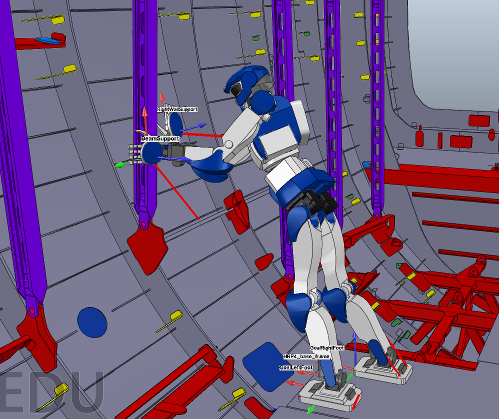
\includegraphics[width=0.6\linewidth]{comanoid.png}
  \caption{HRP-4 applying a desired force on a contact point with its right hand.}
\label{fig:comanoid}
\end{figure}

\paragraph{Generating postures in highly constrained environment}
In this scenario, we need to find task-compatible postures of the the HRP-4 inside a highly constrained environment, in the sense that many obstacles limit its displacement, and it must avoid collision with them.
The goal is to be able the reach the four corners of a panel of circuit breakers (in green on~\Figref{fig:getafe}) to activate them.
We generated a sequence of steps to reach that panel and then some postures to reach different points of this panel.
In~\Figref{fig:getafe}, we show some extracts of this sequence of postures.
In each of them, the two foot are in planar contact with the ground, alternatively bearing forces, while always respecting the joint, torque limits, collision avoidance, and stability constraints.
On the last posture, the top left corner of the panel is reached with the tip of the right hand of the robot.
\begin{figure}
  \centering
  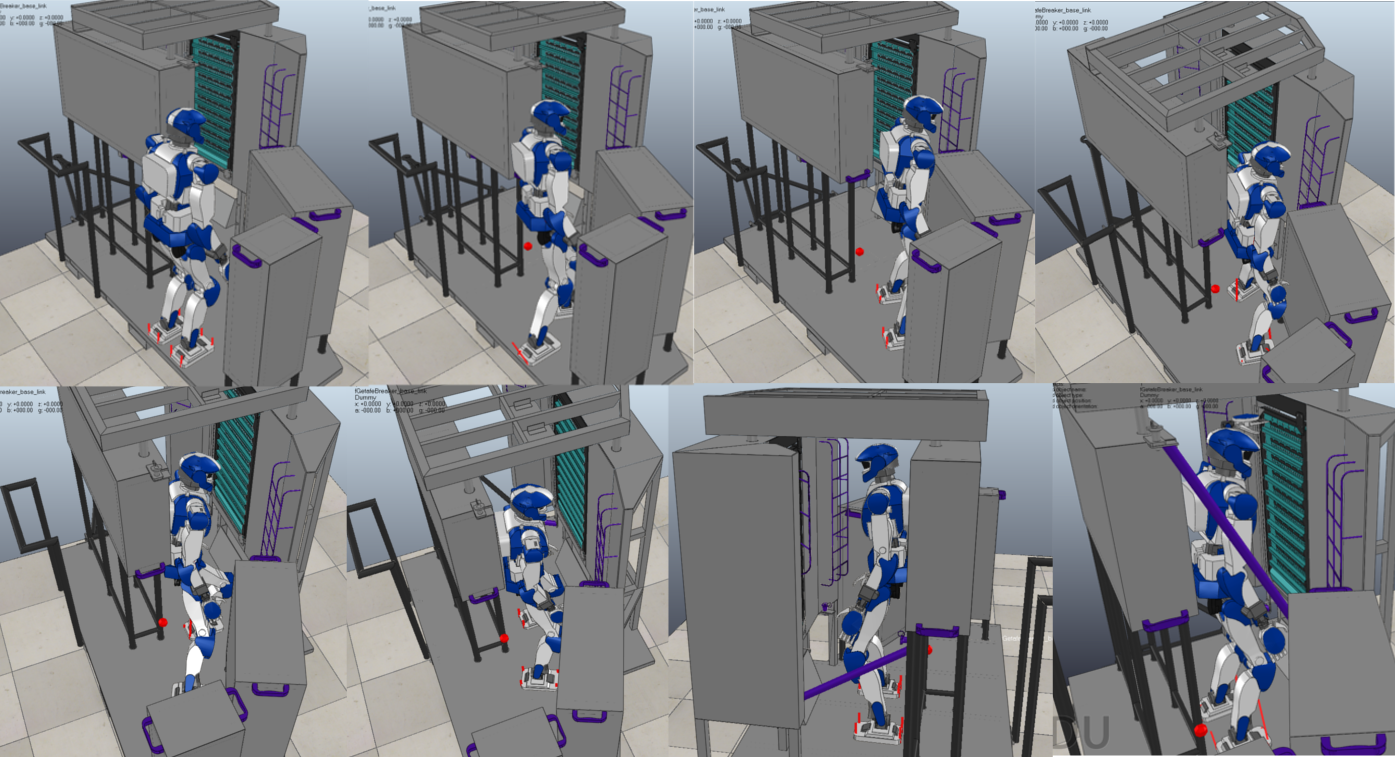
\includegraphics[width=\linewidth]{getafeSequence.png}
  \caption{A sequence of resulting postures with the HRP-4 entering a constrained environments to reach a point on a panel of circuit breakers (in green).}
\label{fig:getafe}
\end{figure}

%%%%%%%%%%%%%%%%%%%%%%%%%%%%%%%%%%%%%%%%%%%%%%%%%%%%%%%%%%%%%%%%%%%%%%%
%                     CONTACT ON NON-FLAT SURFACE                     %
%%%%%%%%%%%%%%%%%%%%%%%%%%%%%%%%%%%%%%%%%%%%%%%%%%%%%%%%%%%%%%%%%%%%%%%

\section{Contact on non-flat surfaces}
\label{sec:contact_on_non_flat_surfaces}

Writing relations between geometric quantities defined in frames allows to describe a large variety of contacts.
%It is especially convenient when the contact points are predefined or when the geometric relations are simple to express, like for the inclusion of 2 convex polygons in each other in the context of a planar contact.
In particular, it allows to write most types of geometric constraints between canonical geometric shapes (point, line, plane).
The most common type of contact constraint encountered is the contact between two surfaces $S_1$ and $S_2$.
The set of equations used to define that type of constraint can be obtained through a frame constraint blocking TZ, RX and RY. Provided that the correct frames are defined, $F_1$ on $S_1$ with $\vec{z_1}$ normal outbound and $F_2$ on $S_2$ with $\vec{z_2}$ normal inbound, the constraint writes as:
\begin{equation}
  \left\{
  \begin{array}{ll}
    \overrightarrow{O_1O_2}\cdot\vec{z_1} = 0\\
    \vec{z_2}\cdot\vec{z_1} \geq 0 \\
    \vec{z_2}\cdot\vec{x_1} = 0 \\
    \vec{z_2}\cdot\vec{y_1} = 0
  \end{array}
  \right.
\label{eq:planar_contact}
\end{equation}

When the two surfaces are flat, a contact between them can be written simply with the set of equations~\Eqref{eq:planar_contact}.
In that case, the quantities involved in the constraint are invariant with the location of the contact point, thus, the equations are valid for any point of the surface (in particular, the normal vector is the same for any point on the surface).
%When it comes to non-flat surfaces, the orientation of the normal vector changes with the location of the contact point, if the contact point is fixed and predefined, the set of equation~\Eqref{eq:planar_contact} can describe the constraint, otherwise, it is not sufficient.
When it comes to non-flat surfaces, the location of the frames used in equations~\Eqref{eq:planar_contact} matters, as the quantities in the constraint equations depend on it.
%(in particular, the normal vector can vary for any point on the surface).

%We propose to describe that type of contact by parametrizing the contact surface, and using an additional variable on which the location of the contact point and its normal vector are parametrized.
%We remind that a contact constraint between $F_1$ and $F_2$ described by eq~\Eqref{eq:planar_contact} requires the full $F_1$ frame and on $F_2$, only the origin and its normal vector are necessary.

%If any(either or both) of the two surfaces in contact is non-plane, finding the exact location of the contact point on the surface is necessary, because then, the normal to the contact is not known in advance.

We propose to add an additional variable $u_S$ to our optimization problem to represent the location of the contact frame on a non-flat surface.
This gives the ability to our solver to choose the optimal contact position on a non-flat surface.
Depending on its shape, the manifold $\mathcal{M}_S$ on which the surface is parameterized can be $\mathbb{R}$, $\mathbb{R}^2$ or $S^2$.
Then we can write the contact constraint on that parametrized frame as follows:
\begin{equation}
\label{eq:param_frame}
  \mathcal{F}(u_S\in \mathcal{M}_S) = \{O(u_S), (x(u_S), y(u_S), z(u_S))\}
\end{equation}
In this section, we successively present several ways to parameterize various non-flat surfaces to generate contacts with them.

%We propose to handle that case by paramaterizing the contact frame on the surface with a variable $u_S$ on a 1 or 2-dimensional manifold $\mathcal{M}_S$ (which, depending on the shape, could be $\mathbb{R}$, $\mathbb{R}^2$ or $S^2$), and adding this variable to our optimization problem.
%Then we can write the contact constraint on that parametrized frame with ease.
%\begin{equation}
%\label{eq:param_frame}
  %\mathcal{F}(u_S\in \mathcal{M}_S) = \{O(u_S), (x(u_S), y(u_S), z(u_S))\}
%\end{equation}

%In that case, an additional set of variables $u_S\in \mathcal{M}_S$ is added the optimization problem and we can desctibe  as well as the constraint set \Eqref{eq:planar_contact} depending on it.

\subsection{Application to plan-sphere contact}
We consider the contact between a body's flat surface $S_B$ of normal $n_B$, with the surface of a sphere $S_s$ of center $c_s$, radius $r_s$, and let $p_s$ and $n_s$ be a point and its normal on $S_s$.
The most general way to express such a constraint is to ensure that $p_s$ is on $S_B$ and that $n_s$ and $n_B$ are opposite.
To do that, we create a variable $v_{S^2}$ on $S^2$, add it to our optimization problem and map $p_S$ and $n_S$ on it.
In our framework, this constraint is expressed exactly as the contact between 2 planar surfaces, once the mappings of $p_s(v_{S^2})$ and $n_s(v_{S^2})$ are done.
In a framework that does not handle manifolds, it would require to setup a specific constraint, ensuring that the distance between $c_s$ and $S_B$ is equal to $r_S$.

In~\Figref{fig:contact_plan_sphere} we show the results obtained by solving a problem where the HRP-2Kai robot has to keep its feet in contact with the ground at fixed positions, touch a sphere with a side of its right wrist and point as far as possible in a given direction $d$ with its left hand, under balance constraints.
The top row of~\Figref{fig:contact_plan_sphere} shows the results for this problem with several different $d$.
%It shows that our optimization algorithm finds an optimal contact point on the sphere to reach its goal as best as possible while satisfying the given constraints.
In every situation, the projection of the CoM is outside the polygon of support, meaning that such postures would not be reached without leaning on the sphere.
\begin{figure}
\centering
  \centering
  \setlength\fboxsep{0pt}
  \setlength\fboxrule{1pt}
  \fbox{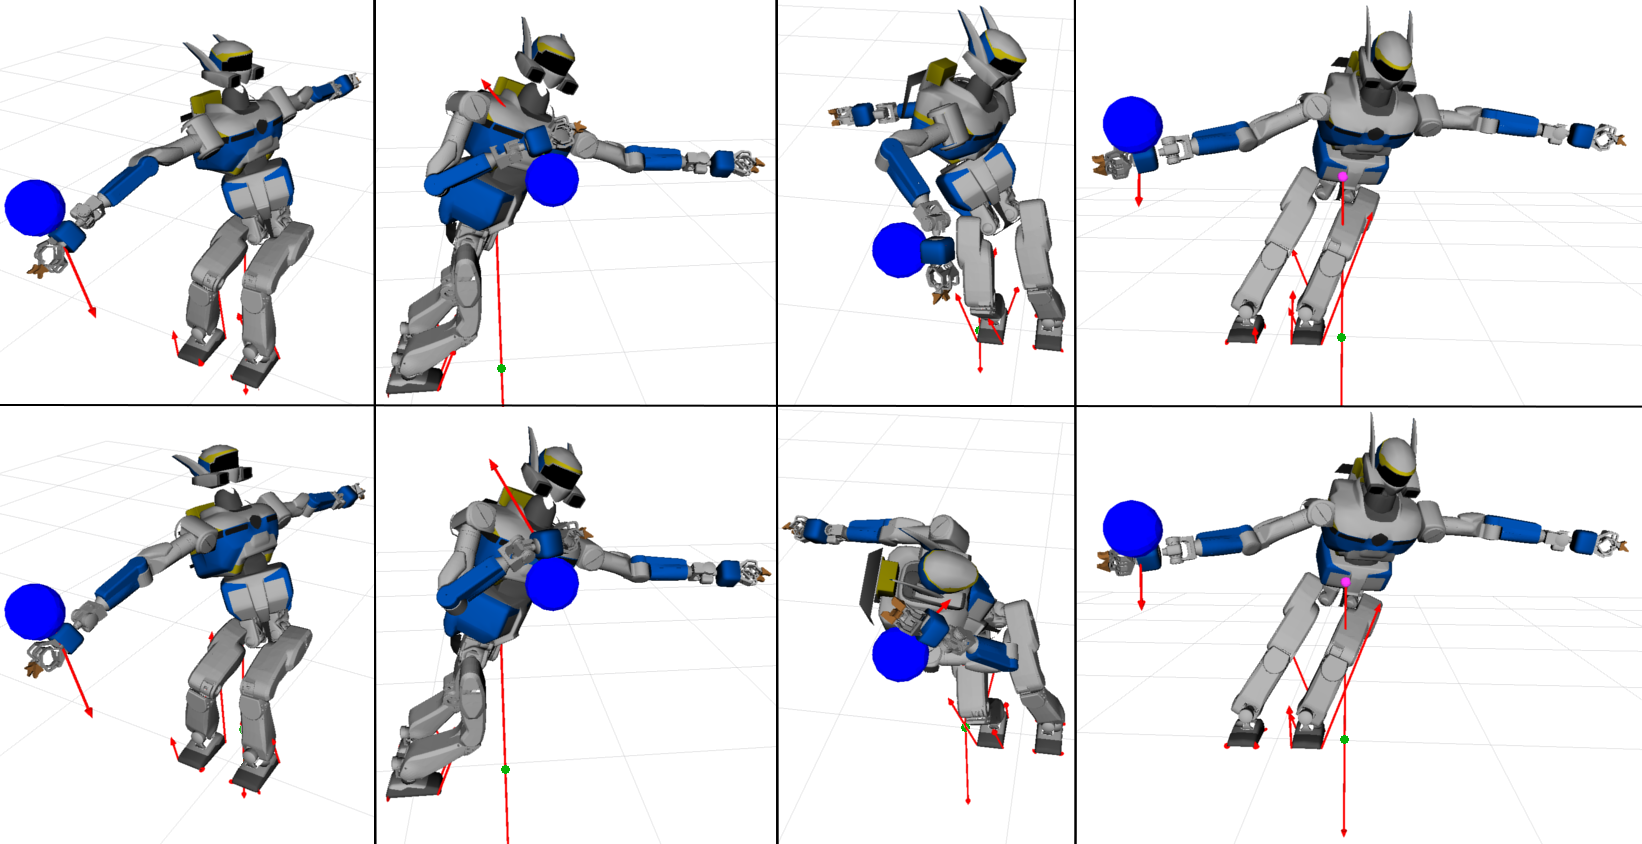
\includegraphics[width=.95\textwidth]{4directionsStrokesWithCoM.png}}
  %\fbox{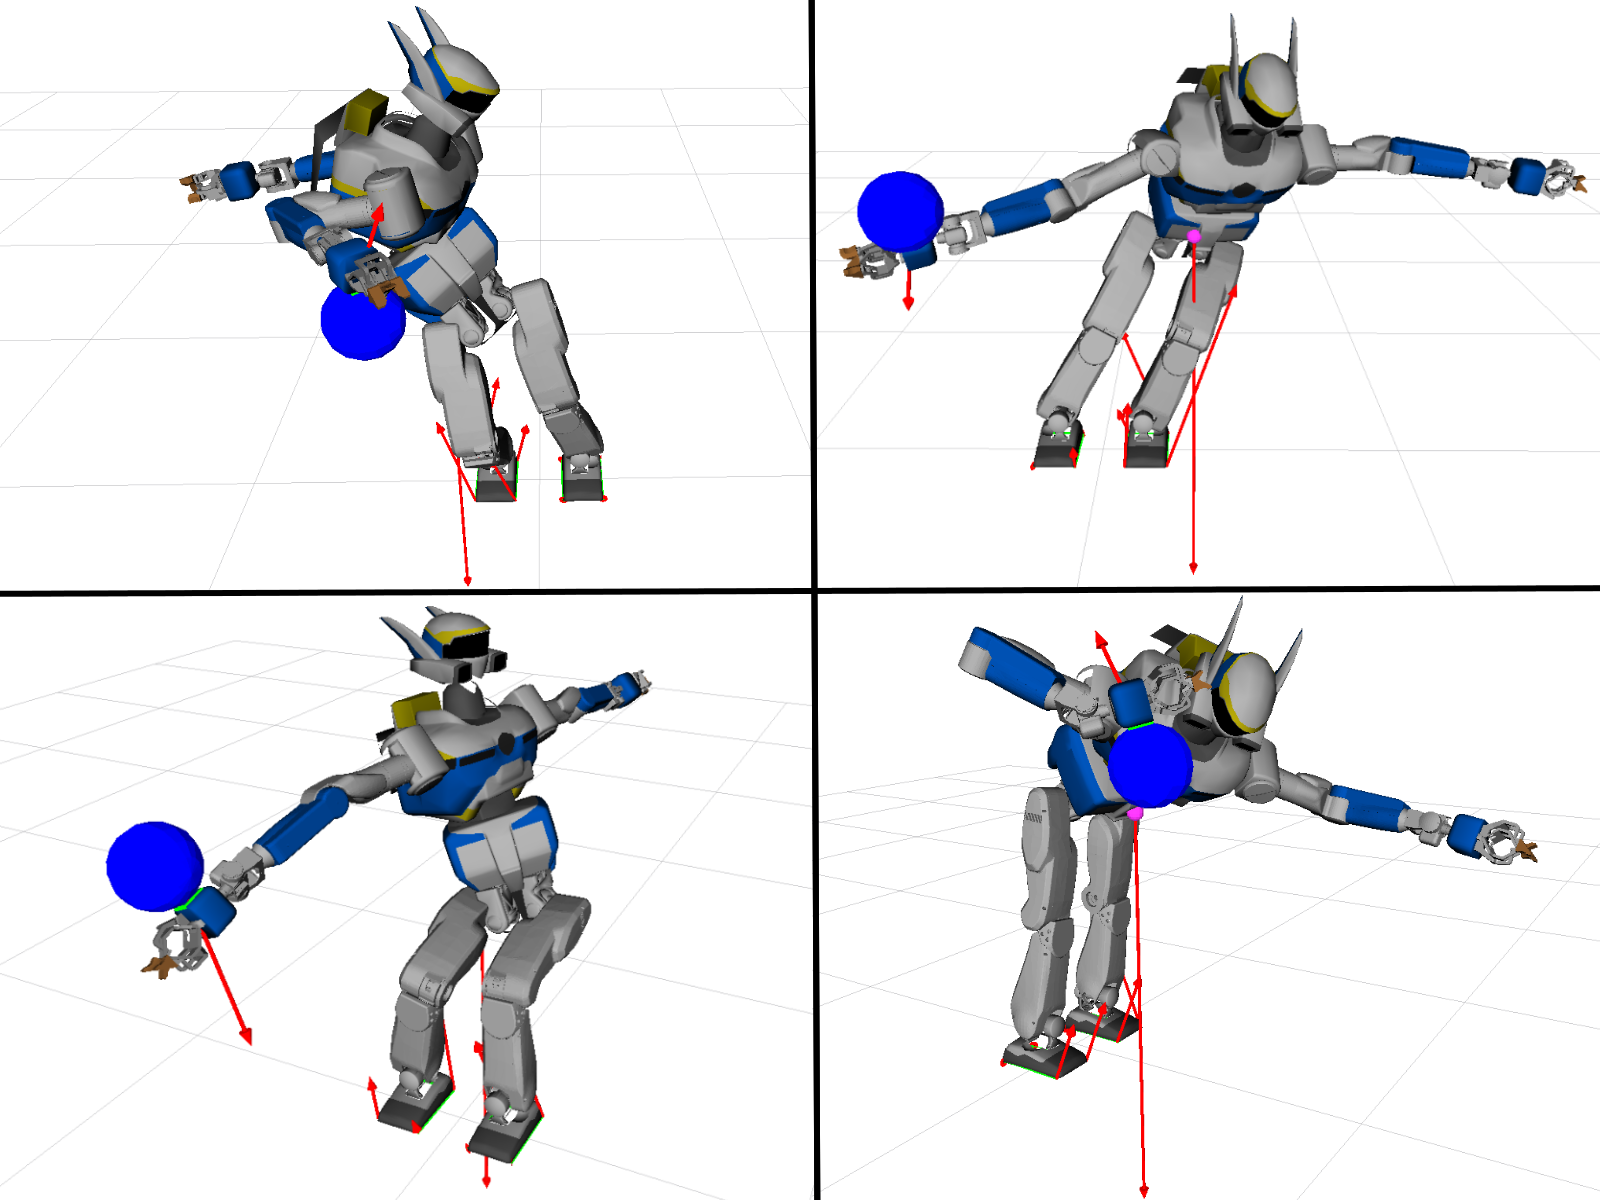
\includegraphics[width=.95\linewidth]{papers/Humanoids2015/figure/contact_plan_sphere_4_directions.png}}}
  \caption{HRP-2Kai leaning on a sphere with its right wrist to point its left gripper as far as possible in 4 cardinal directions.
  Top row: semi-predefined contact; Bottom row: free contact with parametrized wrist.
  Projection of the CoM on the ground (green dots)}
\label{fig:contact_plan_sphere}
\end{figure}

\subsection{Contact with parametrized wrist}

\begin{figure}[!htb]
\centering
  \centering
  \setlength\fboxsep{0pt}
  \setlength\fboxrule{1pt}
  \fbox{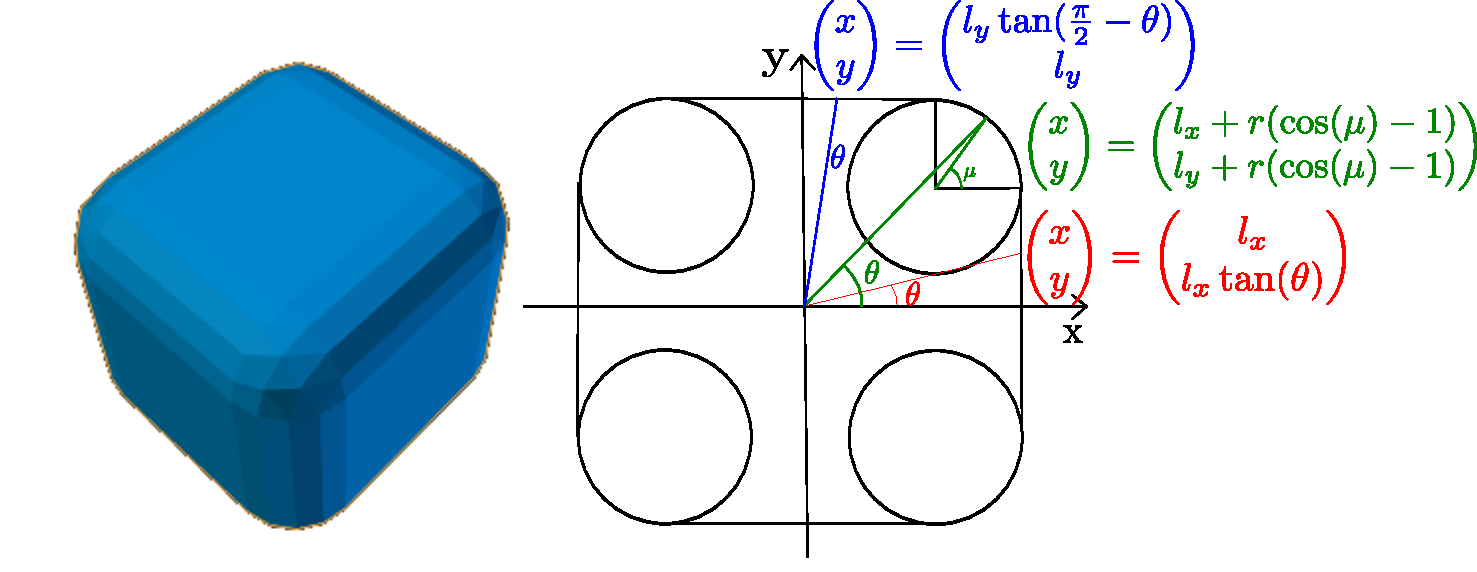
\includegraphics[width=.65\linewidth]{param_wrist_detail.pdf}}
  %\fbox{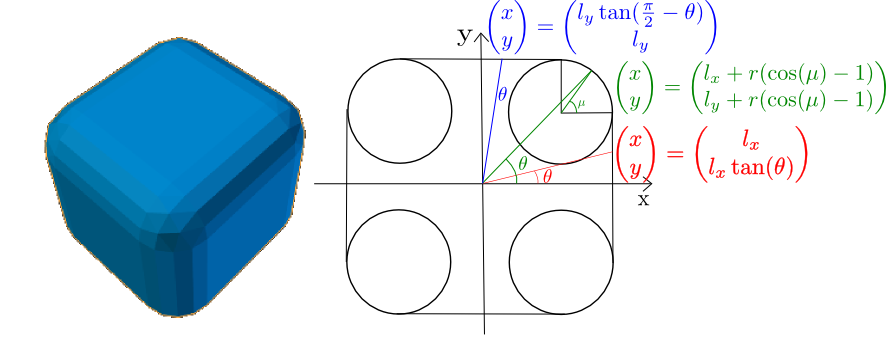
\includegraphics[width=.95\linewidth]{papers/Humanoids2015/figure/param_wrist_detail.png}}
\caption{Parametrization of the wrist of HRP2-Kai}
\label{fig:param_wrist_detail}
\end{figure}

Being able to parametrize the choice for the location of the contact point on the sphere is interesting, but a limitation of this formulation is that the contact point on the wrist of the robot is restricted to one single user-defined face.
Instead, we describe the shape of the wrist body as a parametric function and let the contact point on the wrist as well as its counterpart on the sphere, result from the optimization process.
The section of HRP-2Kai's wrist is a square with rounded edges.
We parametrize this shape as shown in~\Figref{fig:param_wrist_detail}:
we consider the angular coordinate $\theta$ of the point on the section.
It is added as a variable on $\mathbb{R}$ to the problem.
The shape of the quarter of section $[0;\pi/2]$ is a succession of a vertical line, a quarter of a circle and a horizontal line.
This pattern is repeated for the 3 other quarters.
The equations are given in~\Figref{fig:param_wrist_detail}.
In our framework, we define the function describing the shape of the wrist, create a frame parametrized by that function and then define the contact between that frame and the point and the normal on the sphere.
This formulation not only is very easy to implement but most importantly, allows for richer posture generations.
The optimization algorithm chooses the contact point on the sphere as well as the contact point on the wrist, which leads to a wider accessibility range, and a better optimization of the cost function.

The bottom row of~\Figref{fig:contact_plan_sphere} displays the results of this simulation for the robot pointing in 4 directions.
Notice that on the 2nd and the 4th (pointing forward and to the left) images, the results for the 2 types of models are nearly identical, whereas in the 1st and 3rd images, different faces of the wrist have been chosen (On the 1st, the wrist is rotated by $180^{\circ}$, and $90^{\circ}$ on the 3rd).
In these 4 cases, the contact with parametrized wrist gives a better value of the objective function (the left hand points further).
This observation scales:
we solved this problem for 5000 random pointing directions, and in average, the contact with parametrized wrist allows to reach 5mm further.
The success rate of the solver is $98.5\%$ in the parametrized wrist case against $99.9\%$ when the face is fixed.
The numbers of iterations are the same.

%Also, that kind of formulation makes it easier for the user to generate satisfactory postures, as he does not need to specify the plan contact surface anymore.
This method is certainly scalable, and can be used for any kind of humanoid robot and environment.
Yet, it requires having a parametric equation of the surface.

\subsection{Contact with an object parametrized on the unit sphere}

In this case, we want the HRP-4 robot to carry a cube with its two hands.
The most general way to do it is to select a face of the cube for each contact and to enforce the contact between that face and the hand's surface.
We propose to approximate the cube with a superellipsoid and to parametrize the resulting shape on $S^2$, thus adding a variable on $S^2$ to our problem.
The implicit equation of a superellipsoid is $S(x,y,z) = 0$, with
\begin{equation}
  S(x,y,z) = {\left( \left|\frac{x}{A}\right|^r + \left|\frac{y}{B}\right|^r\right)}^\frac{t}{r} + \left|\frac{z}{C}\right|^t - 1
  \label{eq:super_ellipsoid}
\end{equation}

A point in $S^2$ is represented by a vector $v=(x,y,z)$ in $\mathbb{E} = \mathbb{R}^3$.
To a given unit vector $v$ we associate a point $\alpha v$ on the surface of the superellipsoid by solving $S(\alpha v) = 0$ for $\alpha$.
At this point, the normal is given by $\dfrac{\nabla S(\alpha v)}{\left\|\nabla S(\alpha v)\right\|}$ which simplifies into $\dfrac{\nabla S(v)}{\left\|\nabla S(v)\right\|}$.
%It returns the intersection between any unit vector and the surface of the super ellipsoid.
%Also we generate a similar function that returns the normal of the intersection point.
Given this parametrization, we write a contact constraint between the frame of the hand of the robot and the point and normal on the surface of the superellipsoid.

In~\Figref{fig:hrp4_cube} we present some results for a posture generation problem with manipulation: On the left side, the feet are free to move on a sphere, and, on the right side, the left foot position is fixed and the right foot is free to move on the ground.
The hands must be in contact with the cube.
The cube is free to move (parametrized by $\mathbb{R}^3 \times SO(3)$) and has it own set of Euler-Newton equations, which must be fulfilled.
%On the accompanying video, one can observe how the contact points on the cube evolve along with the optimization.
%For each contact with the cube, a variable on $S^2$ is added to the problem to parametrize the contact point.
%Each hand is in contact with a point and normal on the cube.

\begin{figure}
\centering
  \centering
  \setlength\fboxsep{0pt}
  \setlength\fboxrule{1pt}
  \fbox{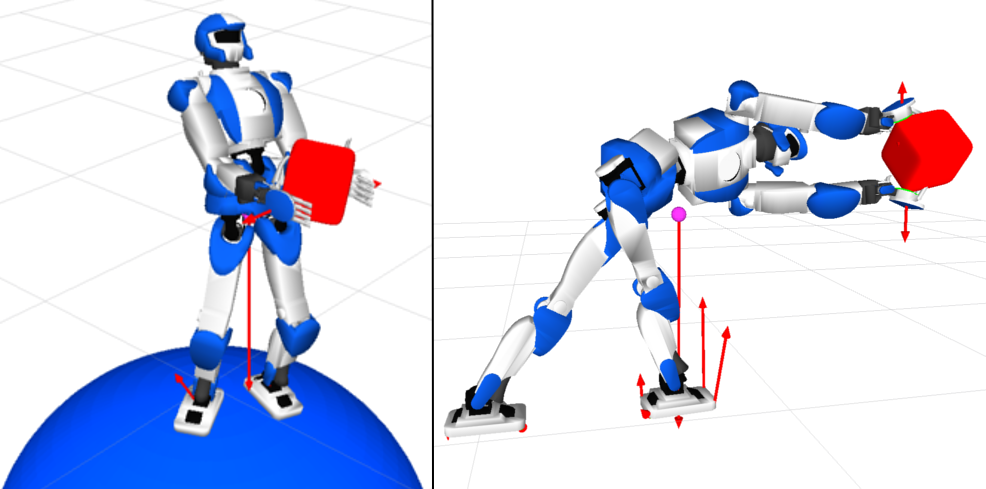
\includegraphics[width=.8\linewidth]{hrp4CubeOnSphere.png}}
\caption{HRP-4 carrying a 2kg cube.
Left: the objective function is to maintain the cube at a given position.
Right: it is to put the cube as far as possible in a given direction}
\label{fig:hrp4_cube}
\end{figure}

\section{Contact with Complex Surfaces}
\label{sec:contact_with_complex_surfaces}

We have presented some methods to formulate contact constraints with parameterized surfaces.
The surfaces that we used so far could all be approximately represented by closed-form equations (sphere, superellipsoid, wrist of HRP-2).
%We showed that to generate contacts between a body of a robot and simple geometric surfaces (sphere, superellipsoid, wrist of HRP2) we can devise some ad hoc parametrization of the surface and write constraints on the resulting approximated surface.
This is sufficient to tackle a large number of interesting scenarios, especially for robots in structured environment~\cite{vaillant:humanoids:2014} \cite{vaillant:autonomousrobots:2016}.
However, contacts with more complex objects are needed too, for unstructured environment or for manipulating objects.

To work with derivative-based optimization algorithms, such as SQP or Interior Points, the functions involved in the optimization problem need to be at least $C^1$ and gradients must be full rank at the solution (for ensuring constraints qualification, see~\cite{nocedal:book:2006}).
Since the contact point can be anywhere on our parametrized surface, the gradients must be full rank everywhere.

In the previously presented parametrizations of typical geometric shapes (sphere, superellipsoid...) those continuity requirements are not a problem.
But for a given object, a parametrization of its surface is rarely available, especially a parametrization conforming with the continuity requirements.
On the contrary, we usually have an approximation of the object as a mesh.

We can consider two types of surface parametrizations, the surfaces of closed topology, like a sphere, which are a large part of the objects of interest in our application, that we parametrize on $S^2$ (because there is no diffeomorphism between the unit sphere and a subset of $\mathbb{R}^2$) and the surfaces of open topology, that generally can be parametrized on $\mathbb{R}^2$.
The problem of finding a parametrization satisfying the continuity requirements exists for both of those when the surface's representation comes as a mesh.

In~\cite{escande:icra:2016}, we provide a systematic way to obtain a parametric surface closely approximating a mesh and meeting the continuity requirements mentioned above, for a large class of objects, namely star-convex objects.
To that end, we combine the use of Catmull-Clark subdivision surfaces with a tailored ray casting algorithm, and propose an efficient and robust numerical method to evaluate a point, a normal and their derivatives at a given set of parameters.

The Catmull-Clark algorithm is used to create a smooth surface modeling a given \emph{control mesh}.
It iteratively subdivides a control mesh by following a set of rules.
The limit surface of this subdivision process is called the Catmull-Clark Surface (CCS), see~\Figref{fig:CCIterations}.
\begin{figure}
\centering
  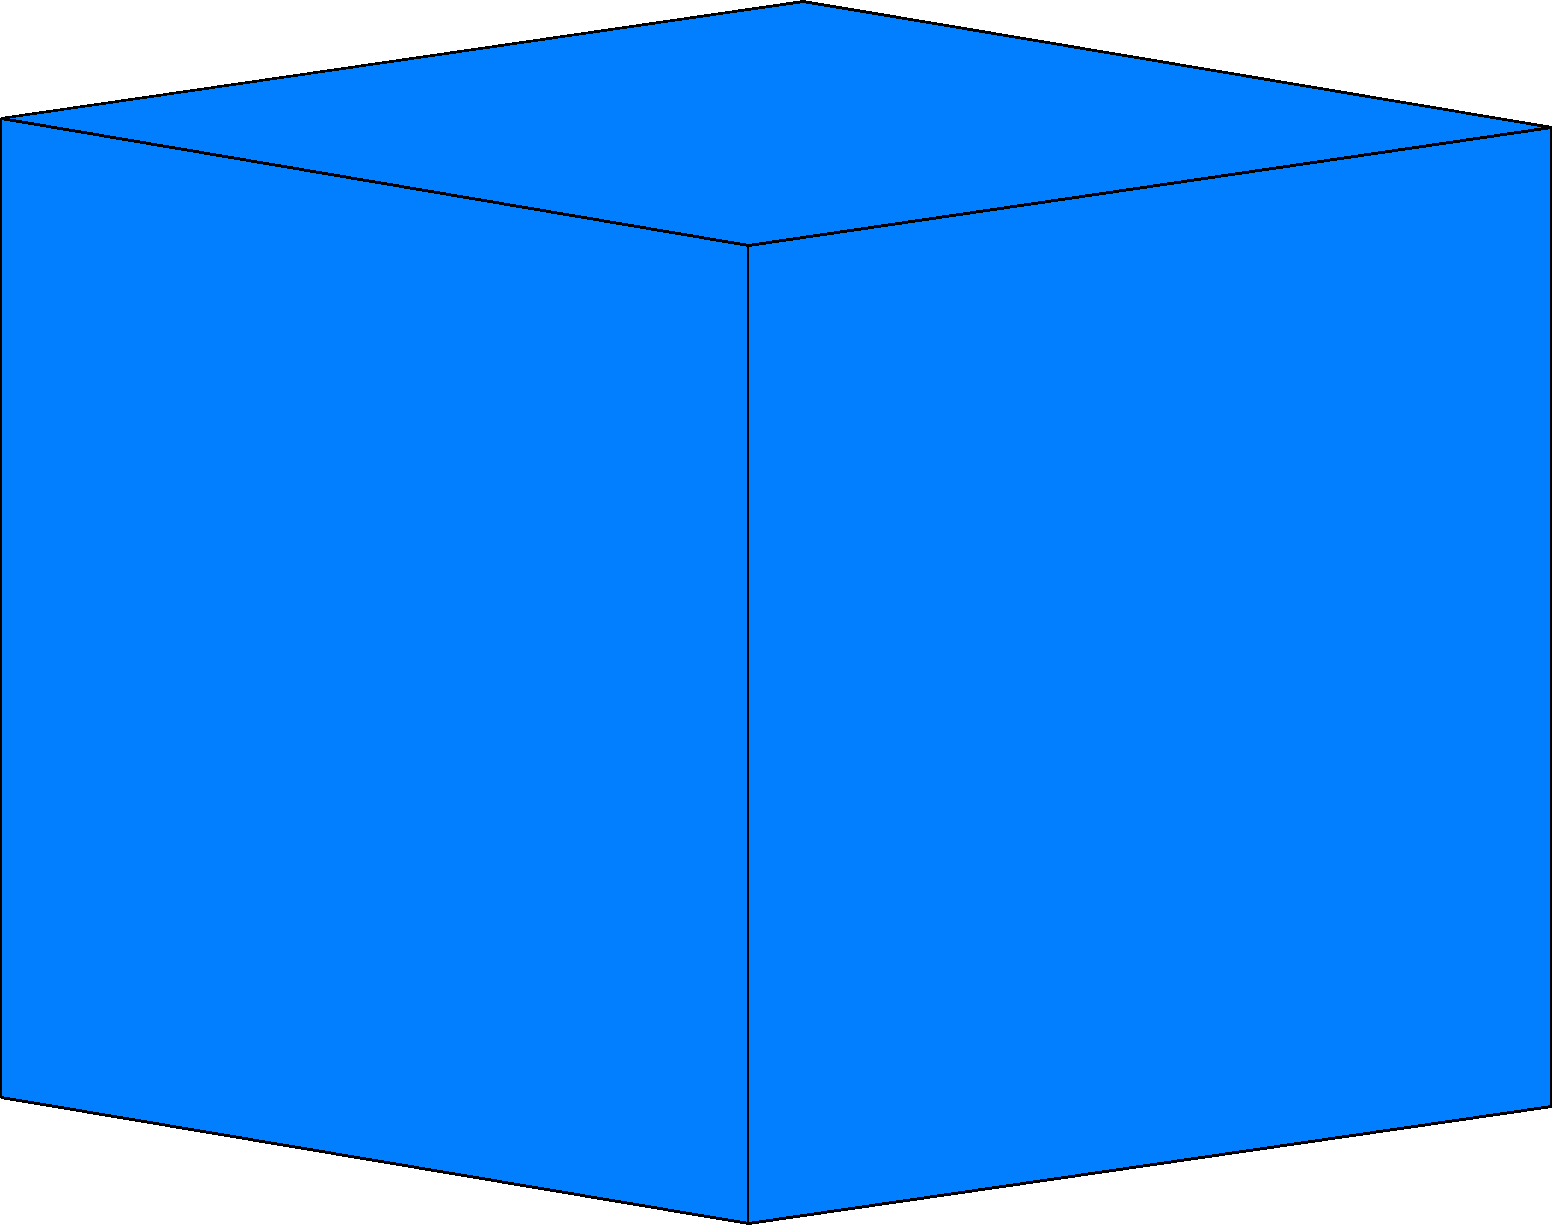
\includegraphics[height = 2cm]{cube1.png}
  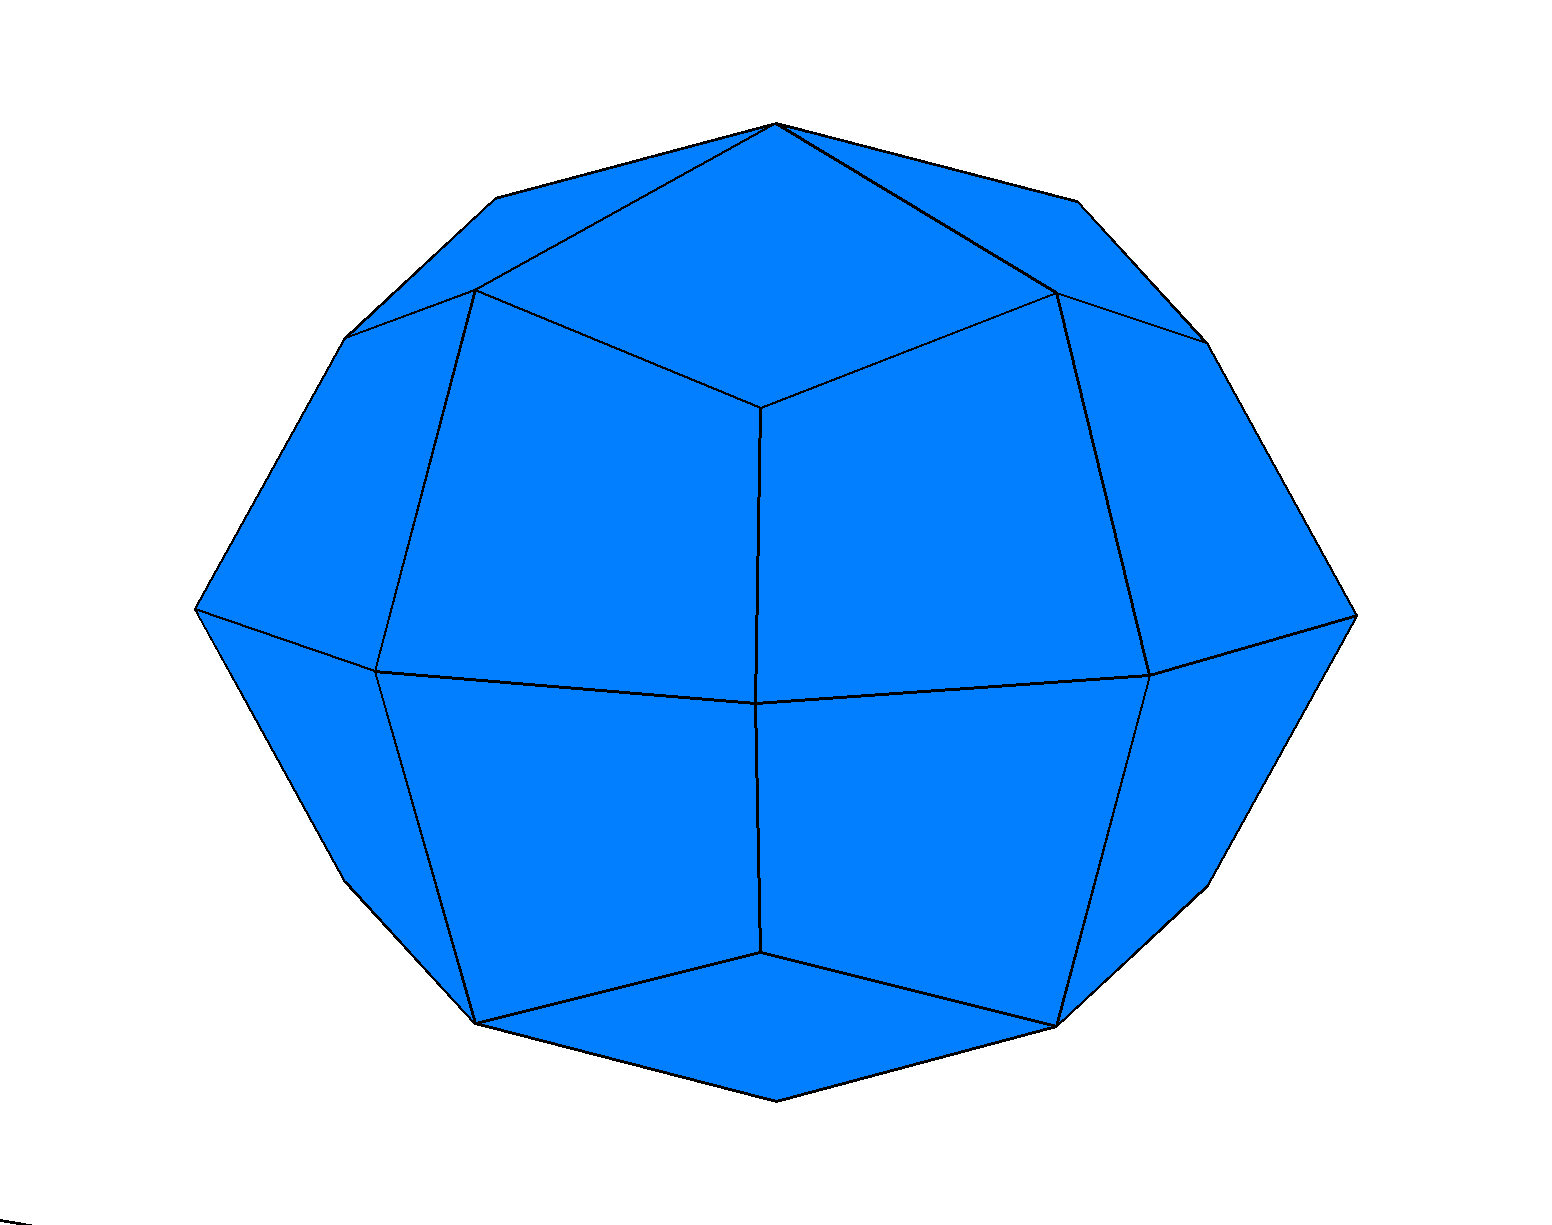
\includegraphics[height = 2cm, trim=20pt 0 50pt 0, clip]{cube2.png}
  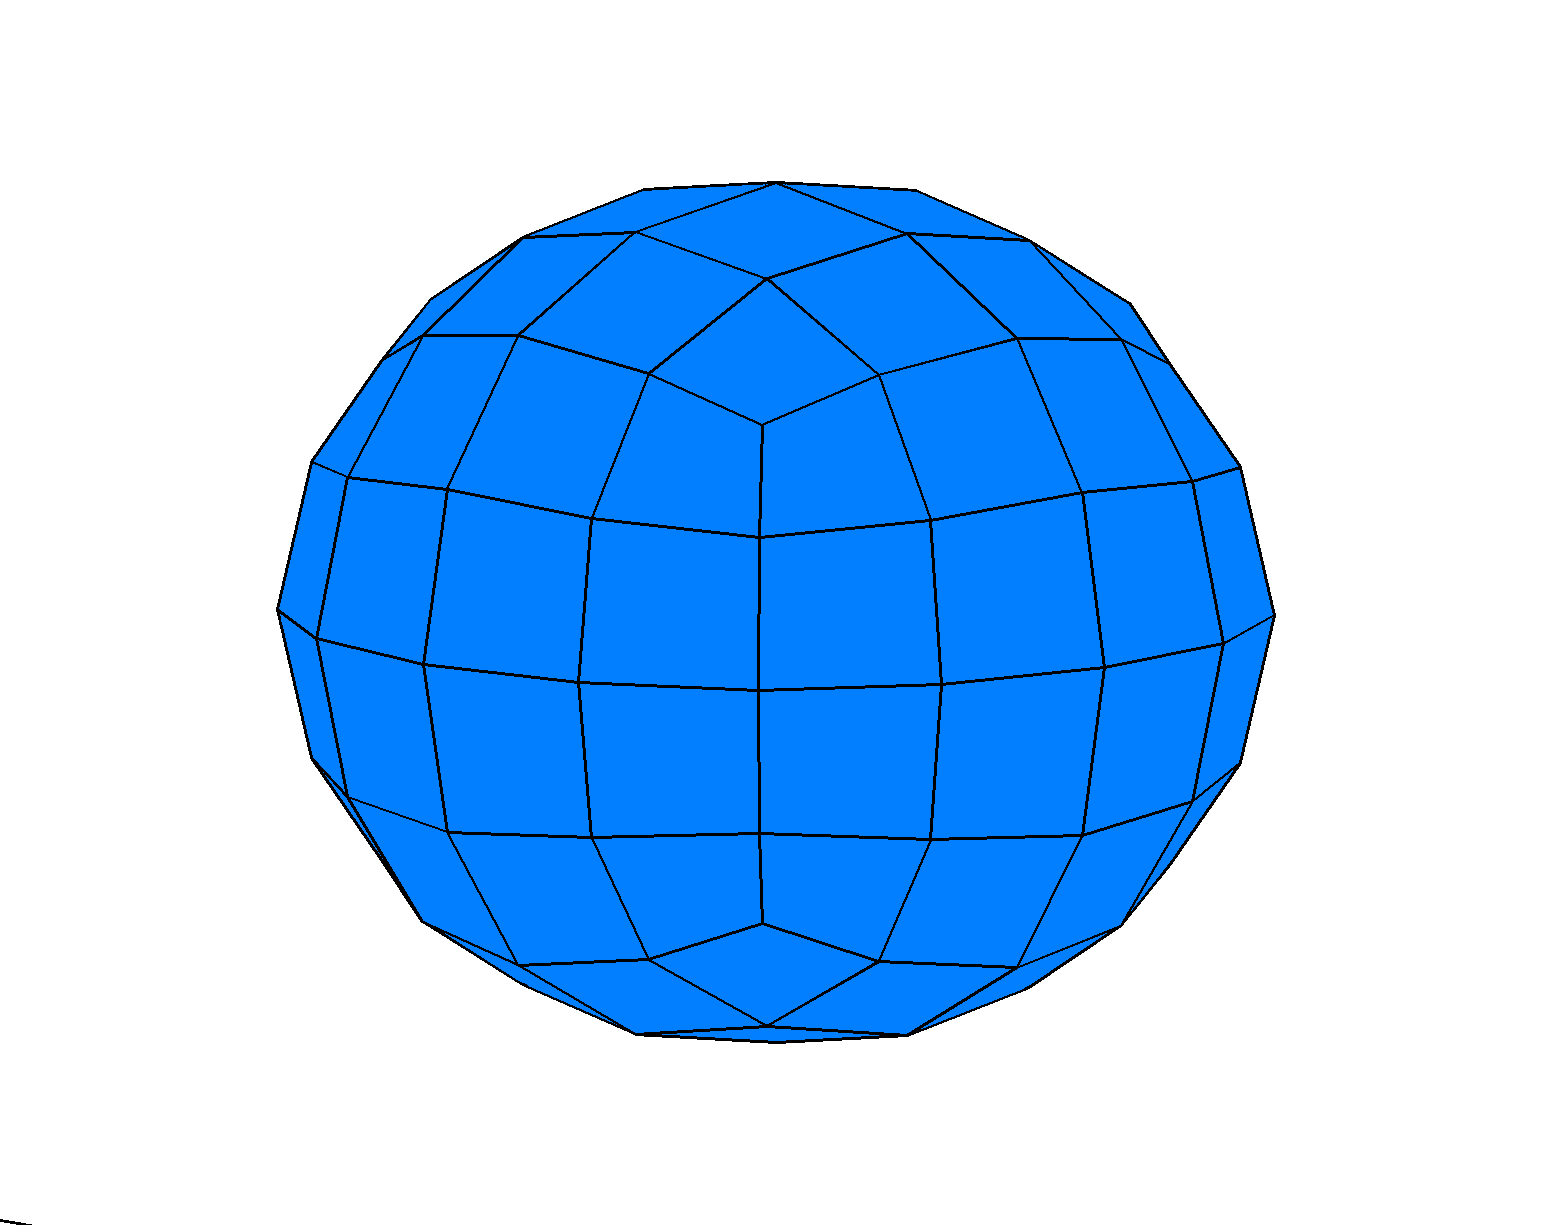
\includegraphics[height = 2cm, trim=50pt 0 50pt 0, clip]{cube3.png}
  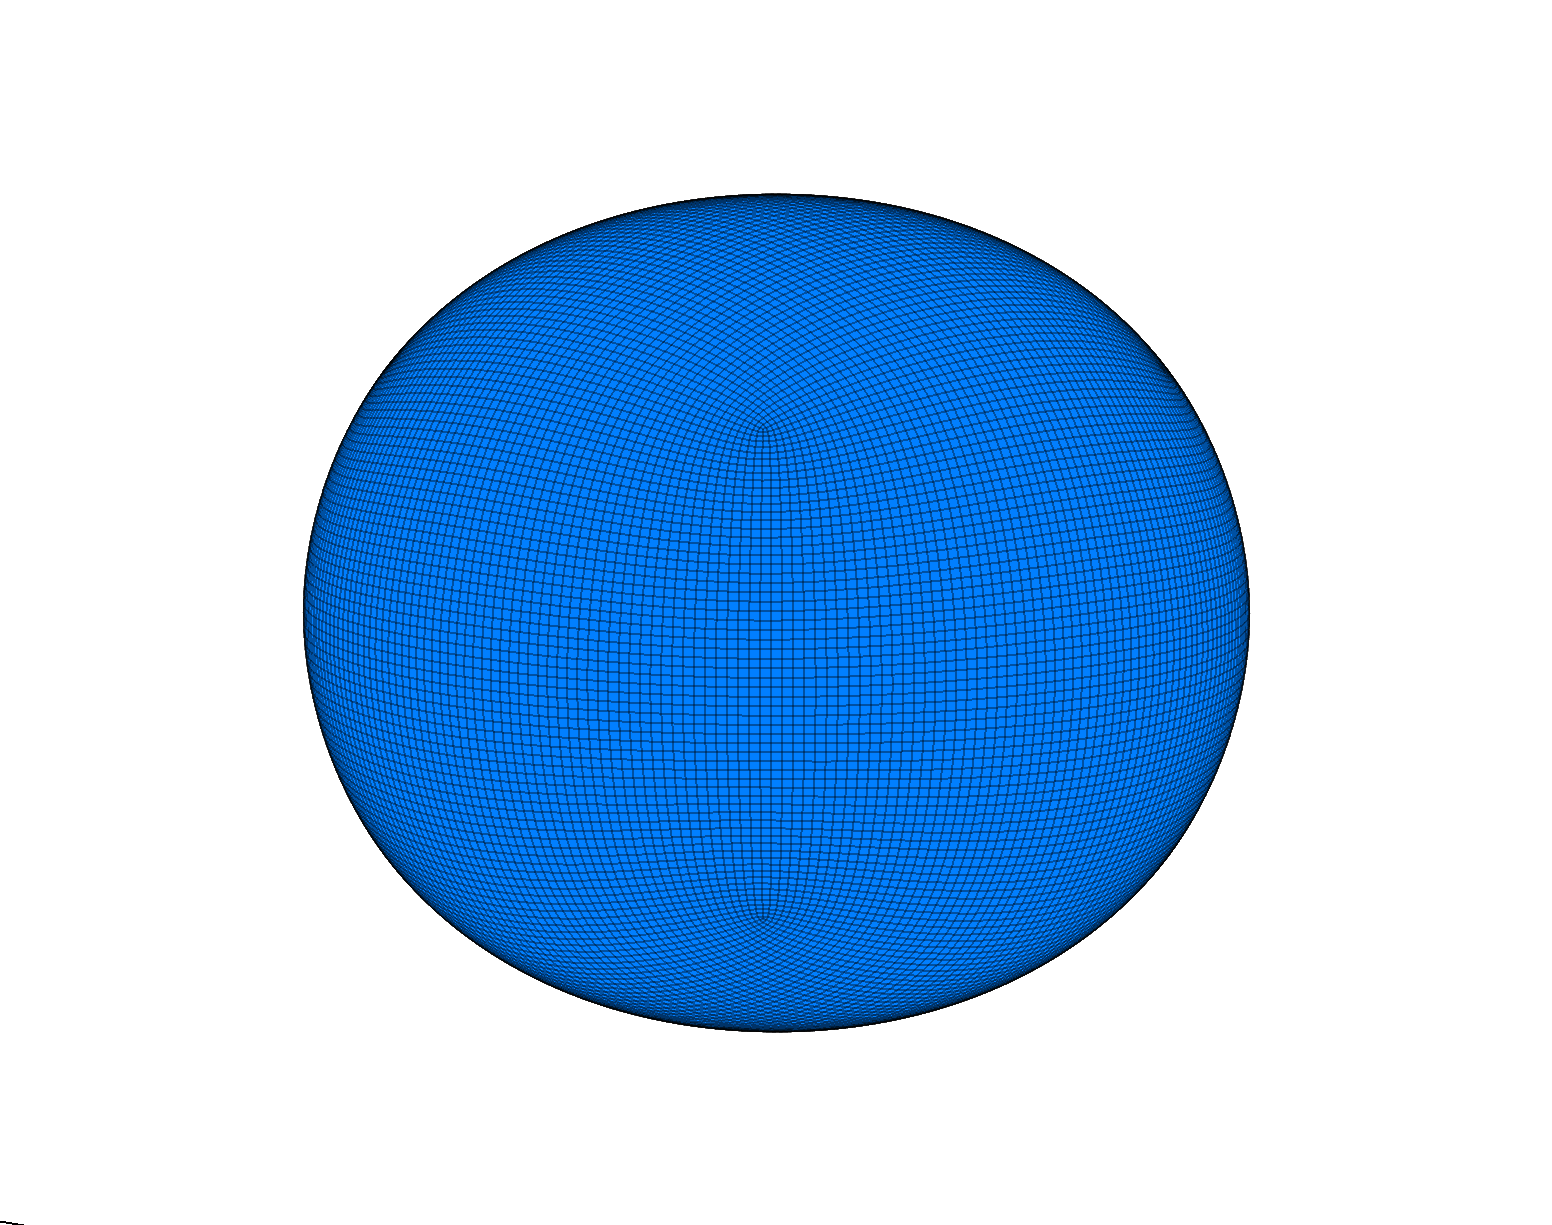
\includegraphics[height = 2cm, trim=50pt 0 50pt 0, clip]{cube4.png}
\caption{Several Catmull-Clark subdivisions of a cube. From left to right: original mesh, after $1$, $2$ and $6$ iterations}
\label{fig:CCIterations}
\end{figure}
It was shown by Stam in a seminal paper~\cite{stam:siggraph:1998} that points on CCS can be computed by direct analytical formula without explicitly subdividing the control mesh.
A map between each face of the control mesh and the patch of the CCS associated to it $s(u,v)$ can be devised (with $(u,v)$ a 2D parametrization of a face).
To find the point of the CCS associated with a value $d \in S^2$, we use a raycasting algorithm: given $c$, a center point of the star-convex control mesh (a point seeing all the surface of the control mesh), we solve numerically $c+td=s(u,v)$ in $(u,v,t)$ with a Newton method.
This gives us a mapping from $S^2$ to the CCS.
From there, we propose methods to compute the normal to the CCS point associated with an element of $S^2$ and we devise the derivations of both those mappings.

As a result, we get a smooth parametrization of the input mesh that satisfies the continuity requirements.
In~\Figref{fig:CCS}, we show the Catmull-Clark surface (in blue) corresponding to the mesh (in green) of an HRP-2 link, for two different levels of smoothness.
On the right picture, we first apply twice a simple subdivision scheme, before using Catmull-Clark subdivisions, thus obtaining a surface closer to the original mesh but less smooth.
The red line is the image of a great circle of the unit sphere through our parametrization.
\begin{figure}
  \centering
    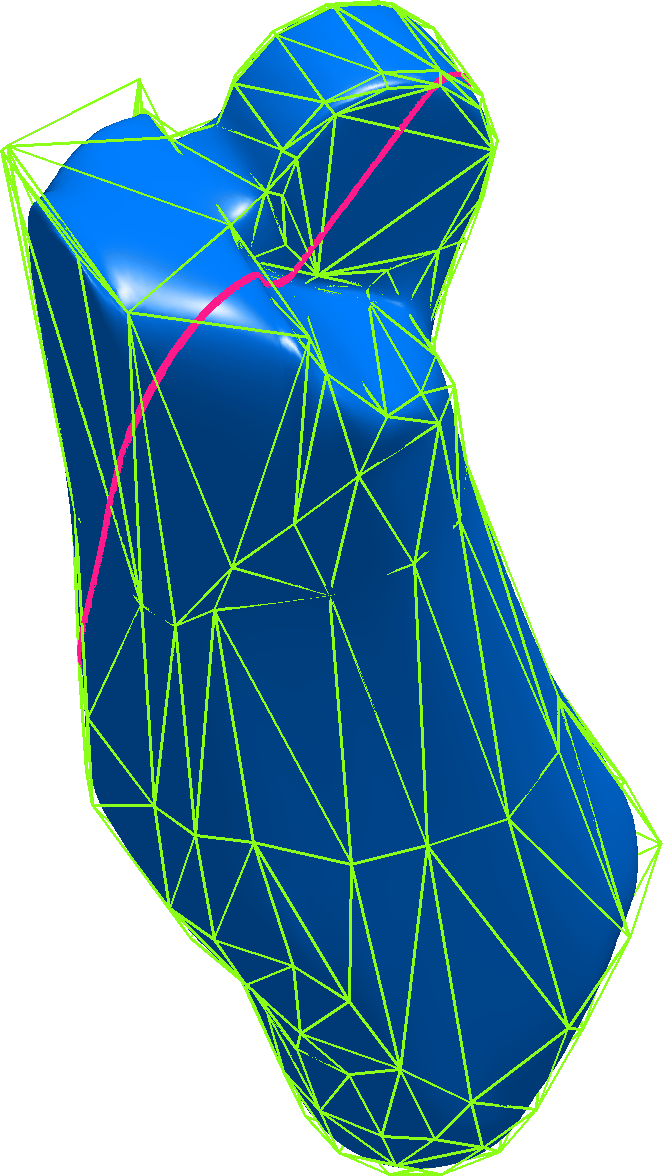
\includegraphics[width = 0.2\paperwidth]{leg3smooth.png}
    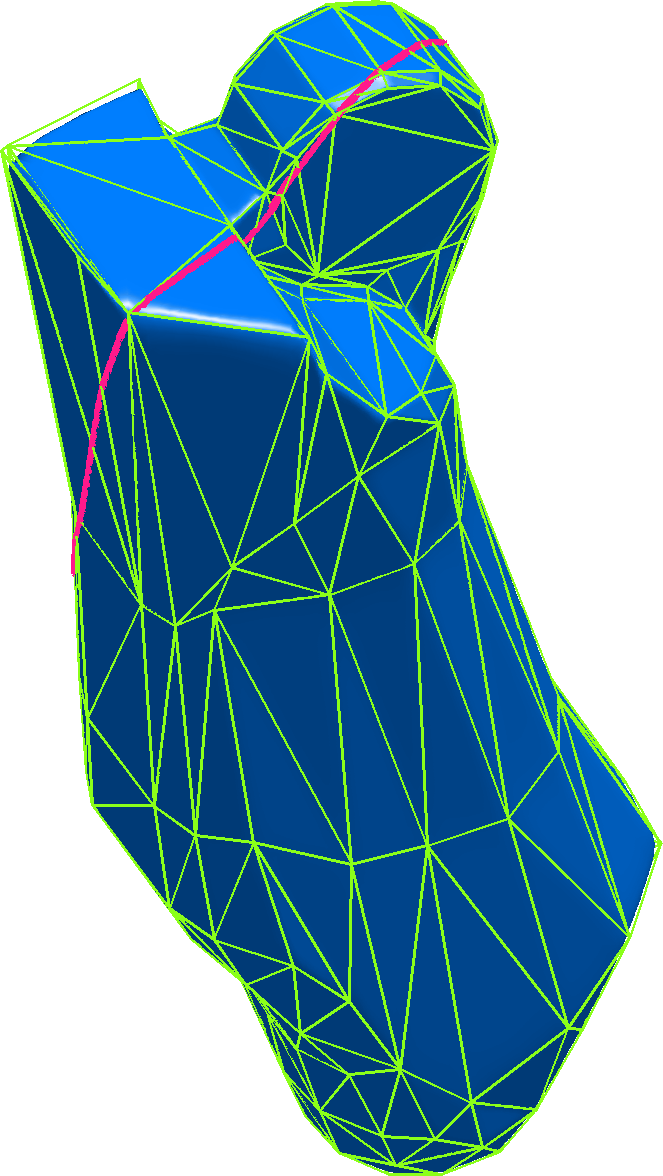
\includegraphics[width = 0.2\paperwidth]{leg3smoothSharp.png}
\caption{Catmull-Clark Surfaces (in blue) approximating the mesh of a link on HRP-2 (in green)}
\label{fig:CCS}
\end{figure}

Because this parametrization respects the continuity requirements for being used efficiently in optimization, we can use it freely in our posture generation problems.

We now show some examples of PG using the proposed approach to generate contacts with complex objects.
We make use of the capacity of our optimization solver to directly work with a variable $d\in S^2$ to parametrize our surfaces.
%When using more classical nonlinear solvers, it is sufficient to take $d$ in $\mathbb{R}^3$ and to add a constraints of unit norm for $d$: the parametrization algorithm do not need a unit $d$ to work, and at the solution, the gradient will be full rank on the null-space of this constraint, which is enough for a good convergence.
%However, working directly on $S^2$ presents several advantages\cite{brossette:Humanoids:2015}.

\begin{figure}
  \centering
    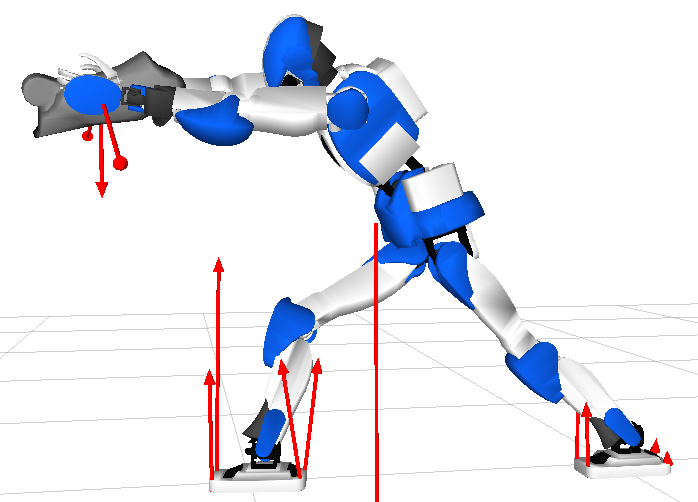
\includegraphics[width = 0.4\linewidth]{hrp4hold.png}
    \includegraphics[width = 0.4\linewidth]{manipulation.png}
\caption{Left: HRP-4 holding an object, modeled with CCS, as far as possible in front of it. The red arrows depict the contact forces and the gravity forces applied on each object. Right: example of grasp generation.}
\label{fig:examples_CCS}
\end{figure}

\begin{figure}
  \centering
    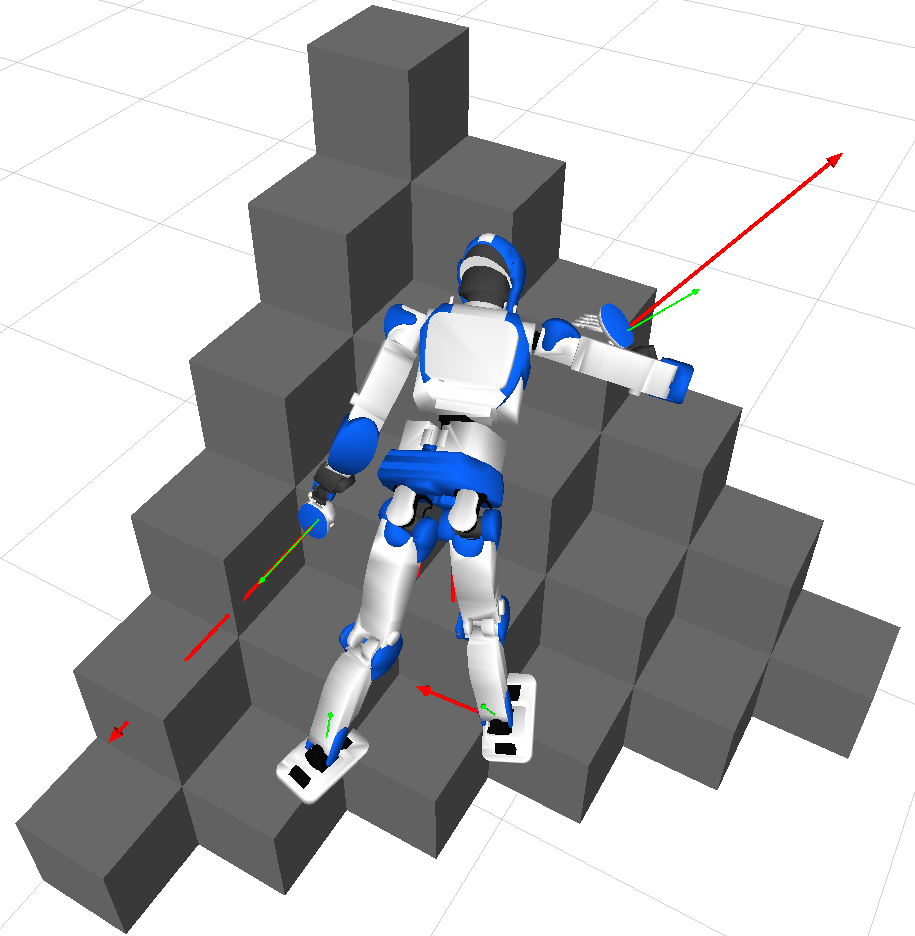
\includegraphics[width = 0.4\linewidth]{cubes.png}
    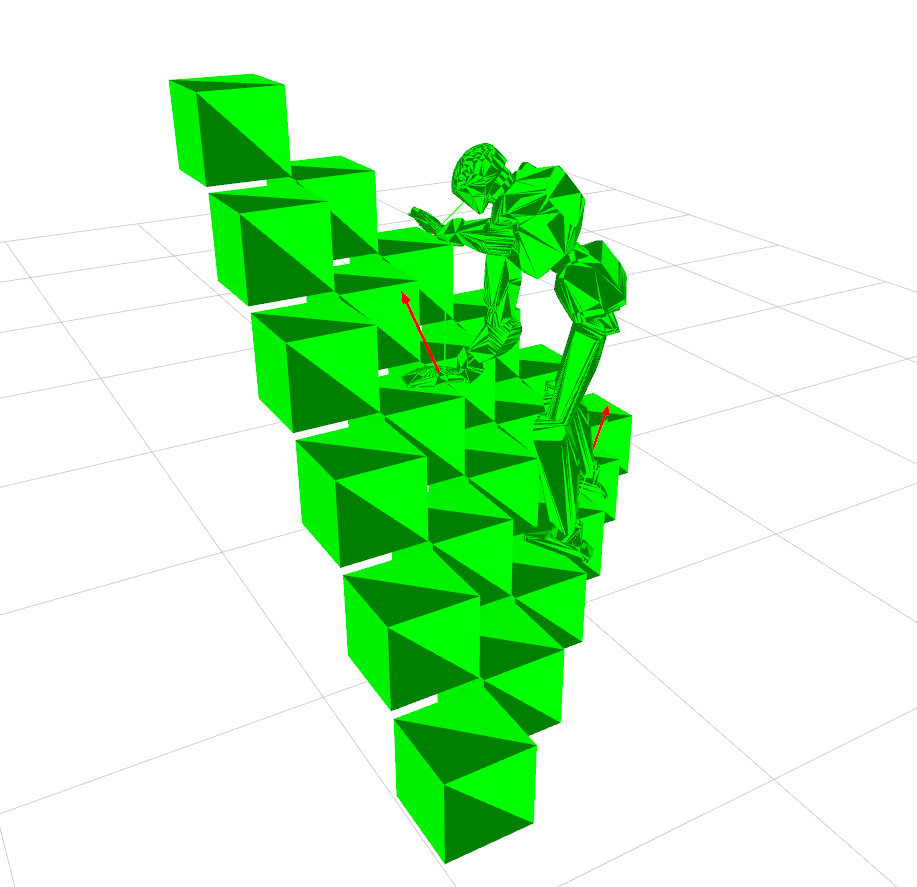
\includegraphics[width = 0.4\linewidth]{cubes_collision.png}
\caption{HRP-4 climbing a pile of cubes modeled as a single object with a single surface. (Right) Convex shapes used for collision avoidance}
\label{fig:HRP4_cubes}
\end{figure}
%\begin{figure}
  %\centering
    %\includegraphics[width=0.8\columnwidth]{img/manipulation.png}
  %\caption{Example of grasp generation.}
  %\label{fig:hand}
%\end{figure}

In the first example (\Figref{fig:examples_CCS}, left), a HRP-4 robot is asked to grasp an object (here a leg part of HRP-2) and to hold it as far as possible in front of it, with the following constraints: contacts must occur between predefined points on the hands of HRP-4 and points free to move on the surface of the object, modeled as a parametric surface with our approach~\cite{escande:icra:2016}; furthermore the robot has to keep its left foot at a given fixed position and has its right foot anywhere on the floor.
The forces applied by the robot on the object must be sufficient to counter the gravity, and the system (robot, object) must be stable with all forces within their friction cones.
Additionally, the robot must stay within its joint limits.
We do not check here for collisions or torque limits.
The solver finds a solution in about $70$ iterations.

Contacts also occur in manipulation.
Actually, manipulation and locomotion are closely related.
Locomotion can be seen as a manipulation of the environment, it is only a matter of reference frame (see~\cite{bouyarmane:ar:2012}).
The second example (\Figref{fig:examples_CCS}, right) demonstrates our PG applied to grasping an object.
The base of the hand is fixed, and the contact points on the fingers are given.
The contact points on the objects are parametrized with our method and are free to move on the entire (approximated) surface of the object: the optimization finds automatically how to grasp the object so as to be able to maintain its stability, taking about $50$ iterations.
Note that the object is non-convex.
%The example is a simple show-case, and we look forward to compare this approach with state-of-the-art methods for grasping.

The third example (\Figref{fig:HRP4_cubes}) involves a stack of cubes on which the robot must stand, using its hands and feet to maintain its stability and respect its torque limits.
The stack is modeled as a single object.
Once again, contact points are fixed on the robot and free on the surface.
The surface is modeled by a single object. That object is not convex, thus it cannot be used as is for collision avoidance.
For collisions, we model the stack of cubes with a set of 21 cubes all slightly smaller than the actual cubes see~\Figref{fig:HRP4_cubes} (Right), and we require the robot to avoid collision with those cubes.
The optimization takes around $115$ iteration to converge to a solution.
Since there is a single surface to contact with, we do not need to specify with which faces, edges or corners the robot needs to be in contact with.
The optimization decides it automatically.
This is a very attractive feature of our approach as it allows to include discrete choices directly into our PG\@.
This can be used to alleviate the work to be done by the user, be it a human or a planning algorithm: the user still has to specify the bodies in contact, but part of the combinatorics relative to the matching of a body with a particular surface or object is handled directly by the PG\@.

\section{Conclusion}
\label{sec:conclusion_ch5}

In this chapter, we presented our approach for formulating a posture generation problem and generating an optimization problem that describes it.
We presented several tools that are meant to simplify this process for the developer, with the automatic variable management, the use of non-Euclidean manifolds and the geometric expressions framework.

Leveraging those tools, we developed methods to formulate constraints involving non-flat surfaces, by adding an extra variable to our optimization problem to parameterize the location of a frame on the surface.
To avoid optimization issues, we make sure that our formulations have satisfying continuity properties.
This addition allows formulating much richer posture generation problems, where the location of a contact on a non-flat surface is abstracted and chosen by the optimization solver.
We were able to use this approach to represent several kinds of surfaces that could be described by closed-form formulas, such as the wrist of HRP-2, a sphere, and a superellipsoid.
We extended that method to approximate surfaces for which the only available representation is a (star-convex) mesh.
This allows formulating constraints on the surface of a very large variety of objects.

In the next chapter, we evaluate the performances of our solver and our posture generator before presenting some use cases and extensions to real world situations.

